\documentclass[a4paper,12pt,twoside]{memoir}

% Castellano
\usepackage[spanish,es-tabla]{babel}
\selectlanguage{spanish}
\usepackage[utf8]{inputenc}
\usepackage[T1]{fontenc}
\usepackage{lmodern} % Scalable font
\usepackage{microtype}
\usepackage{placeins}

\RequirePackage{booktabs}
\RequirePackage[table]{xcolor}
\RequirePackage{xtab}
\RequirePackage{multirow}

% Links
\PassOptionsToPackage{hyphens}{url}\usepackage[colorlinks]{hyperref}
\hypersetup{
	allcolors = {red}
}

% Ecuaciones
\usepackage{amsmath}

% Rutas de fichero / paquete
\newcommand{\ruta}[1]{{\sffamily #1}}

% Párrafos
\nonzeroparskip

% Huérfanas y viudas
\widowpenalty100000
\clubpenalty100000

% Imágenes

% Comando para insertar una imagen en un lugar concreto.
% Los parámetros son:
% 1 --> Ruta absoluta/relativa de la figura
% 2 --> Texto a pie de figura
% 3 --> Tamaño en tanto por uno relativo al ancho de página
\usepackage{graphicx}
\newcommand{\imagen}[3]{
	\begin{figure}[!h]
		\centering
		\includegraphics[width=#3\textwidth]{#1}
		\caption{#2}\label{fig:#1}
	\end{figure}
	\FloatBarrier
}

% Comando para insertar una imagen sin posición.
% Los parámetros son:
% 1 --> Ruta absoluta/relativa de la figura
% 2 --> Texto a pie de figura
% 3 --> Tamaño en tanto por uno relativo al ancho de página
\newcommand{\imagenflotante}[3]{
	\begin{figure}
		\centering
		\includegraphics[width=#3\textwidth]{#1}
		\caption{#2}\label{fig:#1}
	\end{figure}
}

% El comando \figura nos permite insertar figuras comodamente, y utilizando
% siempre el mismo formato. Los parametros son:
% 1 --> Porcentaje del ancho de página que ocupará la figura (de 0 a 1)
% 2 --> Fichero de la imagen
% 3 --> Texto a pie de imagen
% 4 --> Etiqueta (label) para referencias
% 5 --> Opciones que queramos pasarle al \includegraphics
% 6 --> Opciones de posicionamiento a pasarle a \begin{figure}
\newcommand{\figuraConPosicion}[6]{%
  \setlength{\anchoFloat}{#1\textwidth}%
  \addtolength{\anchoFloat}{-4\fboxsep}%
  \setlength{\anchoFigura}{\anchoFloat}%
  \begin{figure}[#6]
    \begin{center}%
      \Ovalbox{%
        \begin{minipage}{\anchoFloat}%
          \begin{center}%
            \includegraphics[width=\anchoFigura,#5]{#2}%
            \caption{#3}%
            \label{#4}%
          \end{center}%
        \end{minipage}
      }%
    \end{center}%
  \end{figure}%
}

%
% Comando para incluir imágenes en formato apaisado (sin marco).
\newcommand{\figuraApaisadaSinMarco}[5]{%
  \begin{figure}%
    \begin{center}%
    \includegraphics[angle=90,height=#1\textheight,#5]{#2}%
    \caption{#3}%
    \label{#4}%
    \end{center}%
  \end{figure}%
}
% Para las tablas
\newcommand{\otoprule}{\midrule [\heavyrulewidth]}
%
% Nuevo comando para tablas pequeñas (menos de una página).
\newcommand{\tablaSmall}[5]{%
 \begin{table}
  \begin{center}
   \rowcolors {2}{gray!35}{}
   \begin{tabular}{#2}
    \toprule
    #4
    \otoprule
    #5
    \bottomrule
   \end{tabular}
   \caption{#1}
   \label{tabla:#3}
  \end{center}
 \end{table}
}

%
% Nuevo comando para tablas pequeñas (menos de una página).
\newcommand{\tablaSmallSinColores}[5]{%
 \begin{table}[H]
  \begin{center}
   \begin{tabular}{#2}
    \toprule
    #4
    \otoprule
    #5
    \bottomrule
   \end{tabular}
   \caption{#1}
   \label{tabla:#3}
  \end{center}
 \end{table}
}

\newcommand{\tablaApaisadaSmall}[5]{%
\begin{landscape}
  \begin{table}
   \begin{center}
    \rowcolors {2}{gray!35}{}
    \begin{tabular}{#2}
     \toprule
     #4
     \otoprule
     #5
     \bottomrule
    \end{tabular}
    \caption{#1}
    \label{tabla:#3}
   \end{center}
  \end{table}
\end{landscape}
}

%
% Nuevo comando para tablas grandes con cabecera y filas alternas coloreadas en gris.
\newcommand{\tabla}[6]{%
  \begin{center}
    \tablefirsthead{
      \toprule
      #5
      \otoprule
    }
    \tablehead{
      \multicolumn{#3}{l}{\small\sl continúa desde la página anterior}\\
      \toprule
      #5
      \otoprule
    }
    \tabletail{
      \hline
      \multicolumn{#3}{r}{\small\sl continúa en la página siguiente}\\
    }
    \tablelasttail{
      \hline
    }
    \bottomcaption{#1}
    \rowcolors {2}{gray!35}{}
    \begin{xtabular}{#2}
      #6
      \bottomrule
    \end{xtabular}
    \label{tabla:#4}
  \end{center}
}

%
% Nuevo comando para tablas grandes con cabecera.
\newcommand{\tablaSinColores}[6]{%
  \begin{center}
    \tablefirsthead{
      \toprule
      #5
      \otoprule
    }
    \tablehead{
      \multicolumn{#3}{l}{\small\sl continúa desde la página anterior}\\
      \toprule
      #5
      \otoprule
    }
    \tabletail{
      \hline
      \multicolumn{#3}{r}{\small\sl continúa en la página siguiente}\\
    }
    \tablelasttail{
      \hline
    }
    \bottomcaption{#1}
    \begin{xtabular}{#2}
      #6
      \bottomrule
    \end{xtabular}
    \label{tabla:#4}
  \end{center}
}

%
% Nuevo comando para tablas grandes sin cabecera.
\newcommand{\tablaSinCabecera}[5]{%
  \begin{center}
    \tablefirsthead{
      \toprule
    }
    \tablehead{
      \multicolumn{#3}{l}{\small\sl continúa desde la página anterior}\\
      \hline
    }
    \tabletail{
      \hline
      \multicolumn{#3}{r}{\small\sl continúa en la página siguiente}\\
    }
    \tablelasttail{
      \hline
    }
    \bottomcaption{#1}
  \begin{xtabular}{#2}
    #5
   \bottomrule
  \end{xtabular}
  \label{tabla:#4}
  \end{center}
}



\definecolor{cgoLight}{HTML}{EEEEEE}
\definecolor{cgoExtralight}{HTML}{FFFFFF}

%
% Nuevo comando para tablas grandes sin cabecera.
\newcommand{\tablaSinCabeceraConBandas}[5]{%
  \begin{center}
    \tablefirsthead{
      \toprule
    }
    \tablehead{
      \multicolumn{#3}{l}{\small\sl continúa desde la página anterior}\\
      \hline
    }
    \tabletail{
      \hline
      \multicolumn{#3}{r}{\small\sl continúa en la página siguiente}\\
    }
    \tablelasttail{
      \hline
    }
    \bottomcaption{#1}
    \rowcolors[]{1}{cgoExtralight}{cgoLight}

  \begin{xtabular}{#2}
    #5
   \bottomrule
  \end{xtabular}
  \label{tabla:#4}
  \end{center}
}



\graphicspath{ {./img/} }

% Capítulos
\chapterstyle{bianchi}
\newcommand{\capitulo}[2]{
	\setcounter{chapter}{#1}
	\setcounter{section}{0}
	\setcounter{figure}{0}
	\setcounter{table}{0}
	\chapter*{\thechapter.\enskip #2}
	\addcontentsline{toc}{chapter}{\thechapter.\enskip #2}
	\markboth{#2}{#2}
}

% Apéndices
\renewcommand{\appendixname}{Apéndice}
\renewcommand*\cftappendixname{\appendixname}

\newcommand{\apendice}[1]{
	%\renewcommand{\thechapter}{A}
	\chapter{#1}
}

\renewcommand*\cftappendixname{\appendixname\ }

% Formato de portada
\makeatletter
\usepackage{xcolor}
\newcommand{\tutor}[1]{\def\@tutor{#1}}
\newcommand{\course}[1]{\def\@course{#1}}
\definecolor{cpardoBox}{HTML}{E6E6FF}
\def\maketitle{
  \null
  \thispagestyle{empty}
  % Cabecera ----------------
\noindent
\includegraphics[width=\textwidth]{cabecera}\vspace{1cm}%
  \vfill
  % Título proyecto y escudo informática ----------------
  \colorbox{cpardoBox}{%
    \begin{minipage}{.8\textwidth}
      \vspace{.5cm}\Large
      \begin{center}
      \textbf{TFG del Grado en Ingeniería Informática}\vspace{.6cm}\\
      \textbf{\LARGE\@title{}}
      \end{center}
      \vspace{.2cm}
    \end{minipage}

  }%
  \hfill\begin{minipage}{.20\textwidth}
    
\includegraphics[width=\textwidth]{escudoInfor}
  \end{minipage}
  \vfill
  % Datos de alumno, curso y tutores ------------------
  \begin{center}%
  {%
    \noindent\LARGE
    Presentado por \@author{}\\ 
    en Universidad de Burgos --- \@date{}\\
    Tutor: \@tutor{}\\
  }%
  \end{center}%
  \null
  \cleardoublepage
  }
\makeatother

\newcommand{\nombre}{Álvaro González Delgado} %%% cambio de comando

% Datos de portada
\title{Implementación del algoritmo TRA-CLUS Mejorado para el análisis de tráfico}
\author{\nombre}
\tutor{Bruno Baruque Zanon y Hector Cogollos Adrian}
\date{\today}

\begin{document}

\maketitle


\newpage\null\thispagestyle{empty}\newpage


%%%%%%%%%%%%%%%%%%%%%%%%%%%%%%%%%%%%%%%%%%%%%%%%%%%%%%%%%%%%%%%%%%%%%%%%%%%%%%%%%%%%%%%%
\thispagestyle{empty}


\noindent
\includegraphics[width=\textwidth]{cabecera}\vspace{1cm}

\noindent D. nombre tutor, profesor del departamento de nombre departamento, área de nombre área.

\noindent Expone:

\noindent Que el alumno D. \nombre, con DNI dni, ha realizado el Trabajo final de Grado en Ingeniería Informática titulado título de TFG. 

\noindent Y que dicho trabajo ha sido realizado por el alumno bajo la dirección del que suscribe, en virtud de lo cual se autoriza su presentación y defensa.

\begin{center} %\large
En Burgos, {\large \today}
\end{center}

\vfill\vfill\vfill

% Author and supervisor
\begin{minipage}{0.45\textwidth}
\begin{flushleft} %\large
Vº. Bº. del Tutor:\\[2cm]
D. nombre tutor
\end{flushleft}
\end{minipage}
\hfill
\begin{minipage}{0.45\textwidth}
\begin{flushleft} %\large
Vº. Bº. del co-tutor:\\[2cm]
D. nombre co-tutor
\end{flushleft}
\end{minipage}
\hfill

\vfill

% para casos con solo un tutor comentar lo anterior
% y descomentar lo siguiente
%Vº. Bº. del Tutor:\\[2cm]
%D. nombre tutor


\newpage\null\thispagestyle{empty}\newpage




\frontmatter

% Abstract en castellano
\renewcommand*\abstractname{Resumen}
\begin{abstract}
El presente proyecto tiene como objetivo el desarrollo de una aplicación web interactiva para la visualización y análisis de trayectorias mediante la implementación del algoritmo de agrupamiento de trayectorias TRACLUS y el estudio de sus variantes. La solución integra herramientas de procesamiento de datos y visualización para facilitar la interpretación de patrones espaciales en trayectorias, con énfasis en eficiencia y aplicabilidad en entornos de Big Data. Se emplearon metodologías ágiles y tecnologías modernas como Dash y scikit-learn para garantizar un diseño modular y adaptable.
\end{abstract}

\renewcommand*\abstractname{Descriptores}
\begin{abstract}
TRACLUS, análisis de trayectorias, agrupamiento, visualización de datos, Dash, scikit-learn, Big Data.
\end{abstract}

\clearpage

% Abstract en inglés
\renewcommand*\abstractname{Abstract}
\begin{abstract}
This project aims to develop an interactive web application for the visualization and analysis of trajectories through the implementation of the TRACLUS trajectory clustering algorithm and the study of its variants. The solution integrates data processing and visualization tools to facilitate the interpretation of spatial patterns in trajectories, focusing on efficiency and applicability in Big Data environments. Agile methodologies and modern technologies such as Dash and scikit-learn were employed to ensure a modular and adaptable design.
\end{abstract}

\renewcommand*\abstractname{Keywords}
\begin{abstract}
TRACLUS, trajectory analysis, clustering, data visualization, Dash, scikit-learn, Big Data.
\end{abstract}


\clearpage

% Indices
\tableofcontents

\clearpage

\listoffigures

\clearpage

\listoftables
\clearpage

\mainmatter
\capitulo{1}{Introducción}

El presente trabajo aborda el desarrollo e implementación de un sistema orientado al análisis de grandes volúmenes de datos geoespaciales mediante técnicas de agrupamiento o \textit{clustering}. En concreto, se ha centrado en el algoritmo TRA-CLUS, diseñado para segmentar y agrupar trayectorias GPS, y en la creación de una aplicación web interactiva que facilite la interpretación y comparación de los resultados obtenidos con diferentes algoritmos de clustering.

El análisis de trayectorias es una tarea fundamental en campos como la movilidad urbana, la gestión del tráfico y la planificación territorial. Sin embargo, la complejidad y el volumen de datos asociados a estas áreas hacen necesario el uso de algoritmos eficientes y herramientas visuales que permitan extraer información útil de manera intuitiva. Este proyecto tiene como objetivo ofrecer una solución integral que combine una implementación optimizada del algoritmo TRA-CLUS con una interfaz visual de fácil uso.

La estructura de esta memoria está diseñada para presentar de manera clara y ordenada el desarrollo del proyecto:

\begin{itemize}
    \item \textbf{Capítulo 1 - Introducción}: Introduce el contexto general del proyecto, sus motivaciones y la organización de esta memoria.
    \item \textbf{Capítulo 2 - Objetivos del Proyecto}: Detalla los objetivos generales, técnicos y personales que han guiado el desarrollo del trabajo.
    \item \textbf{Capítulo 3 - Conceptos Teóricos}: Expone los fundamentos teóricos relacionados con el análisis de trayectorias, el clustering y las técnicas utilizadas en el desarrollo del proyecto.
    \item \textbf{Capítulo 4 - Técnicas y Herramientas}: Describe las tecnologías y herramientas empleadas, justificando su elección y explicando su aplicación dentro del proyecto.
    \item \textbf{Capítulo 5 - Aspectos Relevantes del Proyecto}: Presenta las decisiones clave tomadas durante el desarrollo, los desafíos enfrentados y las soluciones implementadas.
    \item \textbf{Capítulo 6 - Trabajos Relacionados}: Revisa proyectos y estudios previos que guardan relación con este trabajo, destacando sus aportaciones y diferencias con el presente proyecto.
    \item \textbf{Capítulo 7 - Conclusiones y Líneas de Trabajo Futuras}: Resume los resultados alcanzados, las lecciones aprendidas y propone posibles mejoras y extensiones para el proyecto.
\end{itemize}

En conclusión, este proyecto pretende no solo resolver un problema específico del análisis de trayectorias, sino también sentar las bases para futuras investigaciones y desarrollos en el ámbito del Big Data aplicado a datos geoespaciales.

\capitulo{2}{Objetivos del proyecto}

Este apartado explica de forma precisa y concisa cuales son los objetivos que se persiguen con la realización del proyecto. Se puede distinguir entre los objetivos marcados por los requisitos del software a construir y los objetivos de carácter técnico que plantea a la hora de llevar a la práctica el proyecto.

\capitulo{3}{Conceptos teóricos}

\section{Introducción}

En este apartado se presentan los conceptos teóricos fundamentales que permiten comprender el marco conceptual en el que se desarrolla este trabajo. Estos conceptos proporcionan el contexto necesario para el análisis y desarrollo del estudio realizado.

La discusión se centrará en los principios relacionados con el algoritmo TRACLUS, dado que este ha sido el enfoque principal del estudio y representa la mayor complejidad en su implementación y análisis.

\section{Trayectorias GPS}

Las trayectorias GPS se refieren a secuencias de puntos geoespaciales capturados mediante dispositivos de posicionamiento global (GPS). Cada punto de una trayectoria contiene información geográfica, como la latitud, longitud, y, en algunos casos, la altitud y el tiempo asociado. Estas trayectorias son fundamentales para analizar el movimiento de objetos o individuos a lo largo del tiempo y el espacio.

\begin{itemize}
    \item \textbf{Formato típico}: Una trayectoria GPS suele representarse como una lista ordenada de coordenadas \([x, y]\), donde \(x\) corresponde a la longitud y \(y\) a la latitud. Un ejemplo típico es:
    \[
    [[\text{longitud}_1, \text{latitud}_1], [\text{longitud}_2, \text{latitud}_2], \dots]
    \]
    \item \textbf{Origen de los datos}: Estas trayectorias se generan a partir de dispositivos móviles, vehículos, sensores de navegación y otros sistemas de rastreo que capturan posiciones geográficas en intervalos regulares de tiempo.
    \item \textbf{Aplicaciones}: Las trayectorias GPS son esenciales en áreas como la planificación de rutas, el análisis del tráfico, el monitoreo ambiental y la movilidad urbana. También sirven como base para algoritmos de agrupamiento y análisis de datos geoespaciales, como el algoritmo TRA-CLUS.
\end{itemize}

La importancia de las trayectorias GPS radica en su capacidad para modelar patrones de movimiento complejos, facilitando la identificación de tendencias, comportamientos y anomalías en contextos espaciales y temporales. Sin embargo, su análisis presenta desafíos debido a la densidad y complejidad de los datos.


\section{Clustering}

El \textbf{clustering} o agrupamiento es una técnica de aprendizaje no supervisado utilizada para organizar datos en grupos o "clusters" basados en características similares. Cada \textit{cluster} está compuesto por elementos más similares entre sí que a elementos de otros \textit{clusters}. Esta técnica es esencial en análisis exploratorio, permitiendo descubrir estructuras subyacentes en grandes volúmenes de datos y encontrar patrones, sin necesidad de tener etiquetas o categorías predefinidas.

En el contexto de análisis de datos, el clustering se aplica en múltiples áreas como la segmentación de clientes, detección de patrones de comportamiento, agrupación de imágenes y análisis de redes sociales. Entre los métodos de clustering más utilizados en la práctica se incluyen algoritmos basados en densidad y en conectividad, que proporcionan flexibilidad y adaptabilidad para manejar datos complejos y de alta dimensionalidad.

\subsection*{Clustering en el TRA-CLUS}

En el algoritmo TRA-CLUS, el proceso de agrupamiento o \textit{clustering} es una parte fundamental que se utiliza para identificar trayectorias similares basándose en los segmentos generados tras la partición de las trayectorias originales. Para este proyecto, se considera la posibilidad de sustituir el método de agrupamiento original de TRA-CLUS por algoritmos más avanzados o específicos que permitan optimizar los resultados.

La elección de un algoritmo de clustering para TRA-CLUS debe cumplir con las siguientes condiciones clave:
\begin{itemize}
    \item \textbf{Métrica de Distancia Predefinida}: El algoritmo debe ser compatible con una métrica de similitud o distancia previamente calculada, es decir, debe aceptar matrices de distancias precomputadas. Esto es esencial, ya que la similitud entre segmentos en TRA-CLUS se mide previamente y se organiza en una matriz de distancias.
    \item \textbf{Adaptación a Densidades Variables}: Dado que las trayectorias suelen estar distribuidas en áreas con densidades variables, el algoritmo debe ser capaz de manejar estas diferencias para evitar sesgos en los resultados de agrupamiento.
    \item \textbf{Eficiencia Computacional}: Dado el volumen potencialmente grande de datos en estudios de trayectorias, el algoritmo debe ser computacionalmente eficiente para garantizar tiempos de procesamiento razonables.
\end{itemize}

\subsection*{Algoritmos de Clustering en scikit-learn}

A continuación, se presenta una descripción de los algoritmos de clustering que cumplen las condiciones anteriores de la biblioteca \texttt{scikit-learn} de Python:

\subsubsection*{1. DBSCAN (Density-Based Spatial Clustering of Applications with Noise)}

DBSCAN es un algoritmo basado en densidad que agrupa puntos que están en áreas de alta densidad y considera como ruido aquellos que se encuentran en áreas de baja densidad. Los clusters se forman alrededor de puntos densamente conectados y son identificados por dos parámetros: el radio de vecindad (\(\epsilon\)) y el número mínimo de puntos necesarios (\textit{minPts}) para formar un cluster. DBSCAN es especialmente útil para datos con formas irregulares y ruido, ya que ignora puntos aislados que no pertenecen a ninguna agrupación significativa.

\subsubsection*{2. OPTICS (Ordering Points To Identify the Clustering Structure)}

OPTICS es una extensión de DBSCAN que aborda el problema de la sensibilidad a la elección de \(\epsilon\). En lugar de identificar clusters individuales directamente, OPTICS produce una ordenación de los puntos que muestra su estructura de densidad subyacente. Esto permite descubrir clusters a múltiples escalas y niveles de densidad, haciendo posible una mayor flexibilidad en la agrupación de datos.

\subsubsection*{3. HDBSCAN (Hierarchical Density-Based Spatial Clustering of Applications with Noise)}

HDBSCAN es una variante jerárquica de DBSCAN que forma clusters de densidad utilizando una estructura jerárquica en lugar de depender de un valor fijo de \(\epsilon\). A diferencia de DBSCAN y OPTICS, HDBSCAN construye una jerarquía de clusters que permite identificar agrupaciones en diferentes niveles de densidad sin requerir parámetros estrictos. Este algoritmo es particularmente útil cuando la densidad de los clusters varía significativamente.

\subsubsection*{4. Spectral Clustering}

Spectral Clustering es un algoritmo de agrupación basado en teoría de grafos y técnicas de álgebra lineal. Utiliza los valores propios de una matriz de similitud de los datos para realizar la agrupación. Este enfoque es particularmente adecuado para datos que presentan estructuras de clusters no lineales o formas complejas. Spectral Clustering convierte el problema de agrupación en uno de corte de grafos, dividiendo el conjunto de datos en \textit{k} clusters minimizando la similitud entre los clusters.

\subsubsection*{5. Agglomerative Clustering}

El \textbf{Agglomerative Clustering} es una técnica jerárquica de clustering donde cada punto comienza como su propio cluster, y los clusters se fusionan iterativamente en función de una métrica de distancia (como la distancia euclidiana, de Manhattan, o de enlace promedio) hasta que se alcanza el número deseado de clusters o se completa la jerarquía. Este método es particularmente útil cuando se requiere una representación visual de los clusters en forma de dendrograma.

\subsection*{Comparación de los Algoritmos de Clustering}

Los algoritmos de clustering mencionados se diferencian principalmente en su enfoque de agrupación (por densidad, jerárquico o basado en similitud), su sensibilidad a la elección de parámetros y su capacidad para manejar clusters de diferentes formas y densidades. A continuación, se presenta una tabla comparativa de los algoritmos:

\begin{table}[ht]
\centering
\begin{tabular}{|p{2.2cm}|p{2.2cm}|p{3.7cm}|p{4cm}|}
\hline
\textbf{Algoritmo} & \textbf{Tipo de Clustering} & \textbf{Ventaja Principal} & \textbf{Limitación Principal} \\
\hline
DBSCAN & Densidad & Maneja ruido y clusters de formas arbitrarias & Sensible a la elección de \(\epsilon\) y \textit{minPts} \\
OPTICS & Densidad & Detecta clusters a diferentes niveles de densidad & Complejo de interpretar \\
HDBSCAN & Jerárquico basado en densidad & Sin parámetros estrictos & Computacionalmente costoso \\
Spectral Clustering & Basado en grafos & Captura estructuras complejas & Requiere especificar \textit{k} \\
Agglomerative Clustering & Jerárquico & Ofrece dendrograma jerárquico & Alta complejidad para datos grandes \\
\hline
\end{tabular}
\end{table}

\subsubsection*{Conclusión}

Los algoritmos basados en densidad, como DBSCAN, OPTICS y HDBSCAN, son especialmente útiles para datos con clusters de formas irregulares y en presencia de ruido, aunque requieren ajustes específicos de parámetros o presentan alta complejidad computacional. Por otro lado, métodos como Spectral Clustering y Agglomerative Clustering son más adecuados para datos que exhiben estructuras jerárquicas o formas no lineales, pero a costa de una mayor sensibilidad a la configuración inicial y un mayor costo computacional en datasets grandes.

En el contexto del algoritmo TRA-CLUS, donde la similitud entre segmentos se precomputa y los datos presentan densidades variables, los algoritmos basados en densidad, como HDBSCAN, ofrecen ventajas significativas por su flexibilidad y capacidad para manejar variaciones en los datos sin requerir parámetros estrictos. Sin embargo, la elección del algoritmo debe balancear la precisión de los resultados con la eficiencia computacional, considerando las características específicas de las trayectorias a analizar.


\section{TRACLUS}

TRACLUS \cite{lee2007trajectory} es un algoritmo de agrupación (\textit{clustering}) especializado en datos de trayectorias, diseñado para identificar patrones comunes de movimiento en conjuntos de datos de trayectorias, como rutas de vehículos, movimientos de animales o trayectorias de fenómenos meteorológicos. A diferencia de los algoritmos tradicionales de \textit{clustering} que agrupan puntos individuales, TRACLUS se enfoca en el agrupamiento de trayectorias completas, descomponiendo cada trayectoria en segmentos y detectando patrones comunes en subtrayectorias específicas. Este enfoque es útil en estudios donde los objetos presentan secuencias de movimiento en el espacio y el tiempo, permitiendo identificar similitudes parciales dentro de grandes volúmenes de datos.

\subsection*{Principios y Funcionamiento de TRACLUS}

El funcionamiento de TRACLUS se basa en dos etapas principales: la segmentación de trayectorias y la agrupación de segmentos de trayectorias. Ambas etapas están diseñadas para abordar la naturaleza secuencial y direccional de las trayectorias, empleando un enfoque basado en densidad que permite una identificación precisa de subtrayectorias similares.

\begin{enumerate}
    \item \textbf{Segmentación de Trayectorias}: La primera etapa de TRACLUS es dividir cada trayectoria en segmentos de línea más cortos en función de cambios direccionales o puntos de inflexión. Estos puntos característicos dividen la trayectoria en subtrayectorias que pueden ser más fácilmente comparables. Este paso es crucial porque permite detectar patrones comunes en segmentos específicos, en lugar de requerir una coincidencia exacta en toda la trayectoria.

    \item \textbf{Agrupación Basada en Densidad de Segmentos}: En lugar de agrupar puntos aislados, TRACLUS agrupa segmentos que se encuentran en regiones densas del espacio de trayectoria mediante una adaptación del algoritmo DBSCAN (\textit{Density-Based Spatial Clustering of Applications with Noise}). Esta agrupación basada en densidad identifica áreas de alta concentración de segmentos similares que constituyen patrones de movimiento comunes. Los clusters se forman en áreas de alta densidad de segmentos, separadas por regiones de baja densidad, permitiendo agrupar segmentos que comparten características similares, incluso si otras partes de la trayectoria son diferentes.
    
      \item \textbf{Representación de Trayectorias}:  
    TRACLUS utiliza los \textit{clusters} de segmentos generados para representar patrones comunes de trayectorias. En lugar de visualizar cada segmento individual, los \textit{clusters} se representan mediante trayectorias representativas que resumen las características de todos los segmentos pertenecientes a un mismo grupo. Estas trayectorias representativas se calculan promediando las posiciones y direcciones de los segmentos agrupados, proporcionando una visualización simplificada y efectiva de los patrones de movimiento encontrados.
\end{enumerate}

\subsection*{Métrica de Similitud en TRACLUS}

TRACLUS emplea una métrica de similitud diseñada específicamente para medir la relación entre segmentos individuales, en lugar de comparar trayectorias completas. Esta métrica evalúa la similitud entre segmentos considerando tres aspectos principales:

\begin{itemize}
    \item \textbf{Distancia perpendicular}: Mide la distancia más corta desde un punto de un segmento hasta la línea definida por el otro segmento. Esta medida capta la proximidad entre los segmentos desde una perspectiva geométrica.
    \item \textbf{Distancia paralela}: Evalúa la proyección de un segmento sobre el otro, midiendo cuánto de un segmento está alineado en la misma dirección que el otro. Esto permite identificar segmentos con orientaciones similares.
    \item \textbf{Diferencia en la longitud}: Compara las longitudes de los segmentos, lo que ayuda a identificar similitudes en términos de escala o tamaño.
\end{itemize}

La métrica de similitud en TRACLUS combina estas tres distancias en una medida agregada, lo que permite capturar tanto la proximidad espacial como la alineación y el tamaño relativo entre segmentos. Este enfoque es ideal para analizar conjuntos de datos con trayectorias complejas, ya que facilita la identificación de patrones subyacentes al dividir trayectorias en segmentos más pequeños. Sin embargo, este enfoque también conlleva consecuencias importantes en términos de complejidad computacional. Comparar las tres distancias para cada par de segmentos creados implica que cada una de estas mediciones tiene una complejidad de \(O(n^2)\), donde \(n\) es el número total de segmentos. Esta complejidad cuadrática puede afectar significativamente el rendimiento cuando se trabaja con conjuntos de datos de gran tamaño, haciendo fundamental la optimización de las operaciones de comparación para mejorar la eficiencia general del algoritmo.

A diferencia de otras métricas como DTW (Dynamic Time Warping) o LCSS (Longest Common Subsequence), que se enfocan en medir la similitud entre series temporales completas, la métrica de TRACLUS proporciona mayor flexibilidad al detectar subtrayectorias similares. Esto resulta especialmente útil para aplicaciones que requieren identificar patrones locales dentro de trayectorias extensas y densas.

\subsection*{Ventajas de TRACLUS en el Análisis de Trayectorias}
El algoritmo TRACLUS ofrece varias ventajas que lo hacen adecuado para el análisis de datos de trayectoria:

\begin{itemize}
    \item \textbf{Identificación de Subtrayectorias Similares}: TRACLUS no se limita a identificar patrones en trayectorias completas, sino que permite detectar similitudes en segmentos específicos. Esta capacidad es esencial en contextos donde solo algunas secciones de las trayectorias son comparables, mientras que otras presentan variaciones.
    
    \item \textbf{Adaptación a Escalas Variables}: Aunque TRACLUS es sensible a la densidad debido a su enfoque basado en clustering por densidad, su capacidad para manejar variaciones en la escala de las trayectorias lo hace útil en aplicaciones heterogéneas, como estudios de tráfico o movimientos de fauna en diferentes ecosistemas.
    
    \item \textbf{Selección Automática de Parámetros}: Mediante el uso de heurísticas para definir automáticamente los valores de parámetros clave (como el radio de vecindad $\epsilon$ y el número mínimo de puntos vecinos), TRACLUS reduce la necesidad de ajustes manuales. Sin embargo, la elección adecuada de estos parámetros sigue siendo crucial para garantizar resultados precisos en diferentes conjuntos de datos.
\end{itemize}

\subsection*{Aplicaciones de TRACLUS en la Investigación}
TRACLUS se puede aplicar en múltiples campos de investigación, donde el análisis de patrones de movimiento es fundamental:

\begin{itemize}
    \item \textbf{Biología y Ecología}: Para analizar trayectorias de animales, identificando patrones de comportamiento, rutas migratorias o territorios de caza.
    
    \item \textbf{Meteorología}: Para el estudio de trayectorias de fenómenos climáticos como huracanes, permitiendo identificar patrones comunes en ciertos eventos.
    
    \item \textbf{Gestión del Tráfico y Transporte}: En el análisis de rutas vehiculares, detectando patrones de congestión, flujo de tráfico y rutas populares.
\end{itemize}



\capitulo{4}{Técnicas y herramientas}

\section{Introducción}

En esta sección se presentan las técnicas metodológicas y las herramientas de desarrollo que se han utilizado para llevar a cabo el proyecto. Se han considerado diferentes alternativas de metodologías y herramientas, y se ofrece un resumen de los aspectos más destacados de cada opción, junto con una justificación de las elecciones realizadas.

\section{Python}

Python es un lenguaje de programación versátil y fácil de aprender, ampliamente utilizado en el desarrollo de aplicaciones web, análisis de datos y machine learning. En este proyecto, se han utilizado varias bibliotecas de Python que han enriquecido el desarrollo y la funcionalidad de la aplicación:

\subsection{Dash}

Dash es un marco de trabajo desarrollado por Plotly que permite la creación de aplicaciones web analíticas e interactivas utilizando Python. Es especialmente popular en la comunidad de ciencia de datos y visualización debido a sus características y beneficios:
    
\begin{itemize}
	\item \textbf{Interactividad:} Dash permite crear aplicaciones que responden a las interacciones del usuario, como clics, desplazamientos y entradas de datos. Esto es crucial para el análisis de datos en tiempo real y la visualización interactiva.
	\item \textbf{Integración con Plotly:} Las visualizaciones de Dash se basan en la biblioteca Plotly, que permite crear gráficos complejos y visualizaciones de alta calidad con facilidad. Esto enriquece la presentación de datos y facilita la comunicación de resultados.
	\item \textbf{Composición de componentes:} Dash permite combinar diferentes componentes (gráficos, tablas, controles de entrada) en una sola interfaz, lo que facilita la creación de aplicaciones integrales que ofrecen una experiencia de usuario fluida.
	\item \textbf{Despliegue sencillo:} Las aplicaciones construidas con Dash se pueden desplegar fácilmente en servidores web, lo que permite compartir los resultados del análisis con un público más amplio sin requerir instalación adicional por parte del usuario final.
	\item \textbf{Flexibilidad:} Al estar basado en Python, los desarrolladores pueden aprovechar la amplia gama de bibliotecas disponibles para manipular datos, realizar análisis y crear visualizaciones personalizadas, lo que proporciona gran flexibilidad en el desarrollo de aplicaciones.
\end{itemize}

Dash fue elegido para este proyecto debido a su idoneidad en la integración de visualizaciones interactivas con análisis de datos, permitiendo la creación de una interfaz eficiente y dinámica para los usuarios.

\subsection{scikit-learn}

Scikit-learn es una biblioteca robusta y eficiente para machine learning en Python. Proporciona herramientas de análisis predictivo, clustering y aprendizaje automático supervisado y no supervisado. Los algoritmos y parámetros utilizados en este proyecto incluyen:

\begin{enumerate}
    \item \textbf{OPTICS (Ordering Points To Identify the Clustering Structure):}
    Este algoritmo identifica clusters de diferentes densidades en los datos. Los principales parámetros configurables son:
    \begin{enumerate}
        \item \textbf{Metric:} Define la métrica utilizada para calcular las distancias entre puntos. Las opciones disponibles son:
        \begin{enumerate}
            \item \textbf{euclidean:} Utiliza la distancia euclidiana tradicional.
            \item \textbf{l1:} Calcula la distancia Manhattan.
            \item \textbf{l2:} Similar a euclidean, pero con ajustes para ciertas aplicaciones.
            \item \textbf{manhattan:} Igual que \textit{l1}, mide la distancia entre dos puntos como la suma de sus diferencias absolutas.
            \item \textbf{cosine:} Calcula la similitud basada en el coseno del ángulo entre vectores.
            \item \textbf{cityblock:} Otra forma de describir la distancia Manhattan.
        \end{enumerate}
        \item \textbf{Algorithm:} Selecciona el método para encontrar vecinos más cercanos:
        \begin{enumerate}
            \item \textbf{auto:} Elige automáticamente el método más eficiente según los datos.
            \item \textbf{ball\_tree:} Usa una estructura de árbol espacial para organizar los puntos.
            \item \textbf{kd\_tree:} Similar a \textit{ball\_tree}, pero optimizado para ciertas métricas.
            \item \textbf{brute:} Calcula las distancias directamente, sin estructuras optimizadas.
        \end{enumerate}
        \item \textbf{Max\_eps:} Establece el radio máximo para considerar puntos vecinos.
        \item \textbf{Min\_samples:} Define el número mínimo de puntos necesarios para formar un cluster.
    \end{enumerate}
    
    \item \textbf{DBSCAN (Density-Based Spatial Clustering of Applications with Noise):}
    Este algoritmo agrupa puntos densos mientras ignora ruido. Comparte parámetros con OPTICS:
    \begin{enumerate}
        \item \textbf{Metric:} Igual que en OPTICS.
        \item \textbf{Algorithm:} Igual que en OPTICS.
        \item \textbf{Eps:} Especifica el radio para considerar vecinos.
        \item \textbf{Min\_samples:} Igual que en OPTICS.
    \end{enumerate}
    
    \item \textbf{HDBSCAN (Hierarchical Density-Based Spatial Clustering of Applications with Noise):}
    Este algoritmo extiende DBSCAN para trabajar mejor con datos de densidad variable:
    \begin{enumerate}
        \item \textbf{Metric:} Igual que en OPTICS.
        \item \textbf{Algorithm:} Igual que en OPTICS.
        \item \textbf{Min\_samples:} Igual que en OPTICS.
    \end{enumerate}
    
    \item \textbf{Agglomerative Clustering:}
    Este algoritmo agrupa puntos en una jerarquía utilizando diferentes criterios de vinculación:
    \begin{enumerate}
        \item \textbf{Metric:} Igual que en OPTICS.
        \item \textbf{Linkage:} Determina cómo calcular la distancia entre clusters:
        \begin{enumerate}
            \item \textbf{ward:} Minimiza la varianza dentro de los clusters.
            \item \textbf{complete:} Maximiza la distancia entre puntos más lejanos de clusters diferentes.
            \item \textbf{average:} Calcula la distancia media entre todos los puntos de dos clusters.
            \item \textbf{single:} Minimiza la distancia entre los puntos más cercanos de dos clusters.
        \end{enumerate}
        \item \textbf{n\_clusters:} Especifica el número de clusters deseados en los resultados.
    \end{enumerate}
    
    \item \textbf{Spectral Clustering:}
    Este algoritmo utiliza el espectro del grafo de afinidad para realizar clustering:
    \begin{enumerate}
        \item \textbf{Affinity:} Define cómo construir el grafo de afinidad:
        \begin{enumerate}
            \item \textbf{nearest\_neighbors:} Usa vecinos más cercanos para definir las relaciones.
            \item \textbf{rbf:} Utiliza una función base radial para calcular similitudes.
            \item \textbf{precomputed:} Trabaja con una matriz de afinidad ya calculada.
            \item \textbf{precomputed\_nearest\_neighbors:} Usa vecinos más cercanos predefinidos.
        \end{enumerate}
        \item \textbf{Assign\_labels:} Define el método para asignar etiquetas a clusters:
        \begin{enumerate}
            \item \textbf{kmeans:} Usa el algoritmo K-Means para asignar etiquetas.
            \item \textbf{discretize:} Utiliza discretización para asignar etiquetas.
            \item \textbf{cluster\_qr:} Asigna etiquetas usando descomposición QR.
        \end{enumerate}
        \item \textbf{n\_clusters:} Especifica el número de clusters deseados en los resultados.
    \end{enumerate}
\end{enumerate}

\subsection{Otras librerías}

Además de las bibliotecas principales, se emplearon diversas librerías complementarias que cubrieron necesidades específicas del proyecto. Estas se pueden agrupar en diferentes categorías según su funcionalidad:

\subsubsection{Análisis y manipulación de datos}
\begin{itemize}
    \item \textbf{NumPy:} Una biblioteca fundamental para cálculos numéricos que proporciona soporte para matrices y funciones matemáticas. Es la base de muchas otras librerías de análisis y aprendizaje automático.
    \item \textbf{Pandas:} Ampliamente utilizado para trabajar con datos tabulares, se integra perfectamente con otras bibliotecas como NumPy y GeoPandas, facilitando tareas de limpieza, transformación y análisis de datos.
    \item \textbf{GeoPandas:} Extiende las capacidades de Pandas para trabajar con datos geoespaciales, permitiendo análisis y visualizaciones de datos basados en ubicación.
    \item \textbf{Shapely:} Diseñada para manipular y analizar geometrías en Python, es crucial para realizar operaciones como intersecciones y uniones de formas en análisis geoespacial.
    \item \textbf{pyproj:} Facilita las transformaciones de coordenadas y es esencial para interoperar entre distintos sistemas de referencia espacial.
\end{itemize}

\subsubsection{Visualización de datos}
\begin{itemize}
    \item \textbf{Matplotlib:} Una biblioteca versátil para crear visualizaciones estáticas, animadas e interactivas, esencial para la comunicación de resultados.
    \item \textbf{Contextily:} Permite añadir mapas de fondo a visualizaciones geográficas, mejorando la contextualización e interpretación de datos espaciales.
\end{itemize}

\subsubsection{Gestión de datos y archivos}
\begin{itemize}
    \item \textbf{JSON:} Proporciona herramientas para manipular datos en formato JSON, lo que facilita la interacción con APIs y configuraciones.
    \item \textbf{Zipfile:} Utilizada para gestionar archivos comprimidos ZIP, mejorando la transferencia y almacenamiento eficiente de datos.
    \item \textbf{io:} Ofrece funciones para manejar flujos de entrada y salida, útil para la manipulación de archivos y datos en memoria.
    \item \textbf{Base64:} Facilita la codificación y decodificación de datos en formato Base64, útil para transmitir archivos binarios como imágenes o documentos en formatos textuales.
\end{itemize}

\subsubsection{Optimización y concurrencia}
\begin{itemize}
    \item \textbf{Time y threading:} Herramientas integradas en Python para gestionar temporización y tareas concurrentes, lo que mejora la eficiencia y la capacidad de respuesta de la aplicación.
    \item \textbf{ThreadPoolExecutor y Process (módulos concurrent.futures y multiprocessing):} Estas herramientas permiten ejecutar tareas intensivas de manera concurrente y en paralelo, mejorando el rendimiento general. Se utilizan para evitar bloqueos en el flujo principal y optimizar la ejecución de operaciones costosas en términos de computación.
\end{itemize}



\section{CSS}
Cascading Style Sheets (CSS) es un lenguaje utilizado para describir la presentación de documentos HTML y XML. En este proyecto, CSS se ha utilizado para mejorar la estética y la usabilidad de la interfaz de la aplicación desarrollada en Python con Dash. Las razones para su elección incluyen:

\begin{itemize}
    \item \textbf{Separación de contenido y estilo:} CSS permite mantener el contenido HTML separado de su presentación, lo que facilita el mantenimiento del código y la implementación de cambios en el diseño sin afectar el contenido.
    \item \textbf{Responsividad:} Facilita el diseño responsivo, asegurando que la aplicación se vea bien en diferentes dispositivos y tamaños de pantalla. Esto es crucial para mejorar la accesibilidad y la experiencia del usuario.
    \item \textbf{Personalización:} Proporciona flexibilidad para personalizar la apariencia de la aplicación de manera sencilla, permitiendo la creación de un diseño atractivo y funcional que se alinee con los objetivos del proyecto.
    \item \textbf{Compatibilidad:} CSS es compatible con todos los navegadores modernos, lo que asegura que el diseño se mantenga consistente en diferentes plataformas.
\end{itemize}

Estas herramientas y bibliotecas han sido elegidas por su capacidad para facilitar el desarrollo, mejorar la eficiencia del trabajo y proporcionar funcionalidades que son fundamentales para el éxito del proyecto. Cada una de ellas contribuye a un enfoque integral que permite abordar las necesidades del análisis de datos y la creación de aplicaciones web interactivas.


\section{Texmaker}
Texmaker es un editor de texto multiplataforma para la creación de documentos en \LaTeX. Es una herramienta esencial para la redacción académica y técnica, y ha sido fundamental en la redacción de este trabajo por las siguientes razones:

\begin{itemize}
    \item \textbf{Interfaz amigable:} Proporciona un entorno intuitivo y fácil de usar que facilita la edición de documentos en \LaTeX, incluso para aquellos que son nuevos en el sistema.
    \item \textbf{Compilación rápida:} Permite compilar documentos \LaTeX rápidamente con un solo clic, lo que agiliza el proceso de revisión y mejora la productividad.
    \item \textbf{Herramientas integradas:} Incluye herramientas para la gestión de bibliografías, la inserción de gráficos y tablas, así como un visor PDF integrado que facilita la revisión del documento final.
    \item \textbf{Plantillas y ejemplos:} Ofrece diversas plantillas y ejemplos que ayudan a los usuarios a comenzar rápidamente con sus documentos, promoviendo buenas prácticas en la redacción científica.
\end{itemize}


\section{GitHub}
GitHub es una plataforma de desarrollo colaborativo basada en la web que utiliza el sistema de control de versiones Git. Es ampliamente utilizado en la comunidad de desarrollo de software por varias razones:

\begin{itemize}
    \item \textbf{Control de versiones:} GitHub facilita el seguimiento de cambios en el código, lo que permite a los desarrolladores revertir a versiones anteriores si es necesario. Esto es esencial para la gestión de errores y la mejora continua del software.
    \item \textbf{Integración continua:} GitHub se puede integrar con diversas herramientas de automatización, como GitHub Actions, que facilitan la construcción, prueba y despliegue automático del código, mejorando la eficiencia del flujo de trabajo.
    \item \textbf{Documentación y seguimiento de issues:} Proporciona herramientas para documentar el código y gestionar tareas o problemas a través de un sistema de “issues”, lo que facilita la organización y planificación del desarrollo.
\end{itemize}


\section{Herramientas de control de tareas: Kanban y Scrum}

Para llevar un control efectivo de las tareas y asegurar la evolución continua del proyecto, se han utilizado metodologías ágiles como \textbf{Kanban} y \textbf{Scrum}.

\begin{itemize}
    \item \textbf{Kanban:} Se utilizó Kanban debido a su flexibilidad y enfoque visual. Kanban nos permitió gestionar el flujo de trabajo mediante tarjetas en un tablero visual, donde las tareas se movían de una columna a otra (de "Por hacer" a "En progreso" y "Hecho"). Esto facilitó una vista clara de las tareas pendientes, así como una priorización y reestructuración rápida de las mismas según los requerimientos que surgían.
    
    \item \textbf{Scrum:} Se implementó Scrum en ciclos de trabajo denominados \textit{sprints}, con duraciones de dos semanas. Cada \textit{sprint} comenzaba con una reunión en la que se revisaban en retrospectiva las tareas realizadas el último \textit{sprint} y se planificaban los objetivos y metas para la siguiente reunión. Este ciclo permitió adaptar las prioridades en función de los avances realizados y los desafíos encontrados, proporcionando un proceso estructurado que se ajustó bien a las necesidades de fases más avanzadas del desarrollo.
\end{itemize}

El uso combinado de ambas metodologías facilitó tanto la flexibilidad como la estructura necesarias en diferentes fases del proyecto, contribuyendo a un flujo de trabajo eficiente y orientado a resultados.


\section{Patrón Vista-Controlador}

El patrón Vista-Controlador (MVC, por sus siglas en inglés) es un modelo arquitectónico ampliamente utilizado en el desarrollo de aplicaciones que separa la lógica de negocio, la lógica de presentación y la interacción del usuario en tres componentes distintos: Modelo, Vista y Controlador. En este proyecto, se adoptó una variante adaptada del patrón MVC para organizar y estructurar la aplicación desarrollada con Dash. 

\begin{itemize}
    \item \textbf{Modelo:} Representa la lógica de datos de la aplicación y maneja la interacción con el conjunto de datos, incluyendo el procesamiento de los mismos y su transformación para ser utilizados en la interfaz. Esto incluye las operaciones realizadas con bibliotecas como Pandas y GeoPandas.
    \item \textbf{Vista:} Es la responsable de la presentación visual de la aplicación. En este proyecto, las vistas fueron diseñadas utilizando Dash, con un enfoque en la interactividad y la visualización de datos, haciendo uso de componentes como gráficos y tablas.
    \item \textbf{Controlador:} Actúa como intermediario entre el modelo y la vista. En este proyecto, el controlador gestiona los callbacks de Dash, procesando las entradas del usuario y actualizando la vista en función de los cambios realizados en el modelo.
\end{itemize}

Esta separación de responsabilidades permitió un desarrollo modular, facilitando el mantenimiento y la escalabilidad del proyecto, al mismo tiempo que mejoró la claridad en la organización del código.


\section{Testing: pytest y SonarCloud}

El aseguramiento de la calidad del software es un aspecto crucial en el desarrollo de cualquier proyecto. En este trabajo, se implementaron pruebas automatizadas y herramientas de análisis de calidad del código para garantizar la robustez y el mantenimiento del sistema.

\subsection*{pytest}

pytest es un marco de pruebas para Python que permite escribir casos de prueba de manera sencilla y eficiente. Las razones para su elección incluyen:

\begin{itemize}
    \item \textbf{Simplicidad:} Permite escribir pruebas concisas utilizando una sintaxis clara y legible, lo que reduce el tiempo necesario para desarrollar y mantener los casos de prueba.
    \item \textbf{Cobertura de pruebas:} Facilita la ejecución de pruebas automatizadas para verificar la funcionalidad de diferentes módulos del proyecto, asegurando que los cambios en el código no introduzcan errores.
    \item \textbf{Extensibilidad:} pytest soporta la integración con complementos como \textit{pytest-cov}, que proporciona informes detallados sobre la cobertura de código, ayudando a identificar áreas que requieren pruebas adicionales.
\end{itemize}

En este proyecto, se utilizaron pruebas unitarias y funcionales para validar la entrada y salida de datos, la interacción entre componentes y el correcto funcionamiento de los algoritmos de clustering y visualización.

\subsection*{SonarCloud}

SonarCloud es una herramienta basada en la nube para analizar la calidad del código, identificar vulnerabilidades y mejorar la mantenibilidad del software. Su incorporación al proyecto permitió:

\begin{itemize}
    \item \textbf{Análisis estático de código:} Identificar problemas como código duplicado, complejidad ciclomática y vulnerabilidades de seguridad antes de la ejecución.
    \item \textbf{Integración continua:} Integrar SonarCloud con GitHub para analizar automáticamente los cambios realizados en cada \textit{commit}, proporcionando retroalimentación inmediata sobre la calidad del código.
    \item \textbf{Métricas de calidad:} Generar informes detallados sobre la calidad del código, ayudando a priorizar refactorizaciones y a mantener estándares de desarrollo altos.
\end{itemize}

La combinación de pytest y SonarCloud contribuyó a un enfoque integral para garantizar la calidad del proyecto, reduciendo errores y facilitando la detección temprana de problemas durante el desarrollo.

\section*{Sphinx}

Sphinx es una herramienta de documentación automática que se utiliza principalmente para crear documentación técnica de proyectos de software. Originalmente fue diseñada para la documentación de Python, pero ahora se utiliza en una variedad de lenguajes y proyectos. Sphinx permite generar documentación en varios formatos, como HTML, LaTeX, ePub y PDF, a partir de archivos fuente escritos en reStructuredText (\texttt{.rst}) o Markdown.

Algunas de las características clave de Sphinx son:

\begin{itemize}
    \item \textbf{Documentación basada en texto:} Utiliza un formato de texto plano fácil de escribir y leer (\texttt{reStructuredText}).
    \item \textbf{Soporte para código fuente:} Sphinx puede extraer automáticamente información de código fuente, como funciones y clases, a través de la directiva \texttt{autodoc}.
    \item \textbf{Generación automática de índices y tablas de contenido:} Sphinx crea automáticamente índices de contenido y enlaces internos, lo que mejora la navegación en la documentación.
    \item \textbf{Extensiones y personalización:} Sphinx es altamente extensible, permitiendo agregar funciones personalizadas mediante extensiones.
    \item \textbf{Soporte para múltiples formatos:} La documentación generada se puede exportar a diferentes formatos como HTML, PDF, LaTeX, y más.
\end{itemize}

En resumen, Sphinx es una herramienta poderosa y flexible para la creación de documentación de proyectos, que facilita la integración con el código fuente y la personalización del formato de salida.






\capitulo{5}{Aspectos relevantes del desarrollo del proyecto}

\section{Herramientas de control de tareas: Kanban y Scrum}

Para llevar un control efectivo de las tareas y asegurar la evolución continua del proyecto, se han utilizado metodologías ágiles como \textbf{Kanban} y \textbf{Scrum}.

\begin{itemize}
    \item \textbf{Kanban:} Se utilizó Kanban debido a su flexibilidad y enfoque visual. Kanban nos permitió gestionar el flujo de trabajo mediante tarjetas en un tablero visual, donde las tareas se movían de una columna a otra (de "Por hacer" a "En progreso" y "Hecho"). Esto facilitó una vista clara de las tareas pendientes, así como una priorización y reestructuración rápida de las mismas según los requerimientos que surgían.
    
    \item \textbf{Scrum:} Se implementó Scrum en ciclos de trabajo denominados \textit{sprints}, con duraciones de dos semanas. Cada \textit{sprint} comenzaba con una reunión en la que se revisaban en retrospectiva las tareas realizadas el último \textit{sprint} y se planificaban los objetivos y metas para la siguiente reunión. Este ciclo permitió adaptar las prioridades en función de los avances realizados y los desafíos encontrados, proporcionando un proceso estructurado que se ajustó bien a las necesidades de fases más avanzadas del desarrollo.
\end{itemize}

El uso combinado de ambas metodologías facilitó tanto la flexibilidad como la estructura necesarias en diferentes fases del proyecto, contribuyendo a un flujo de trabajo eficiente y orientado a resultados.

\section{Formación y aprendizaje necesario}

El desarrollo del proyecto requirió adquirir nuevos conocimientos y profundizar en diversas tecnologías y técnicas de análisis. A continuación, se describe la formación llevada a cabo en las herramientas y algoritmos más relevantes.

\subsection{Estudio del algoritmo TRACLUS}

El enfoque principal de este proyecto ha sido estudiar en profundidad el algoritmo \textbf{TRACLUS}, destinando una gran parte de las horas de investigación a comprender su funcionamiento y potencial para el análisis de trayectorias. Este algoritmo se basa en la segmentación y agrupación de trayectorias, permitiendo identificar sub-trayectorias comunes dentro de un conjunto de datos. Esto lo convierte en una herramienta valiosa para descubrir patrones significativos en datos de trayectorias. La investigación incluyó la revisión de artículos académicos y la exploración de cómo ajustar los parámetros de TRACLUS para maximizar su efectividad en el contexto específico del proyecto.

Adicionalmente, se evaluó el uso de una implementación de TRACLUS disponible en una biblioteca externa, explorando su viabilidad y características. Aunque esta versión fue útil para los primeros experimentos, se consideraron también posibles variantes y adaptaciones del algoritmo, con el fin de entender mejor el alcance y la adaptabilidad de TRACLUS.

\subsubsection{Propuesta de variantes de TRACLUS}

Durante el desarrollo del proyecto, se analizaron varias propuestas de variantes del algoritmo TRACLUS que han surgido en estudios recientes. Aunque finalmente no se utilizaron, la investigación detallada de estos derivados fue enriquecedora y ayudó a contrastar enfoques para una implementación eficiente. Las variantes de TRACLUS estudiadas fueron:

\begin{itemize}
    \item \textbf{GTraclus:} Una variante diseñada para ejecutarse en unidades de procesamiento gráfico (GPU), optimizando la eficiencia del algoritmo al aprovechar la capacidad de procesamiento paralelo de las GPUs \cite{gtraclus}.

    \item \textbf{ST-TRACLUS:} Esta versión incorpora una dimensión temporal además de la espacial, permitiendo realizar agrupamientos espaciotemporales de trayectorias, lo cual mejora la calidad del análisis para datos donde el tiempo es una variable relevante \cite{st-traclus}.

    \item \textbf{ND-TRACLUS:} Una extensión de TRACLUS que permite realizar el clustering en espacios de n dimensiones, expandiendo su aplicabilidad a trayectorias de mayor dimensionalidad \cite{nd-traclus}.

    \item \textbf{Neighborhood-Based Trajectory Clustering:} Una alternativa basada en densidad local de vecindad en lugar de densidad global. Este enfoque busca mantener la eficiencia de TRACLUS mientras reduce la necesidad de múltiples parámetros de entrada.

    \item \textbf{Adaptive Trajectory Clustering based on Grid and Density (ATCGD):} Un método que introduce una cuadrícula y criterios de densidad para el análisis de patrones móviles, buscando reducir la complejidad computacional y la carga de trabajo en la calibración de parámetros, especialmente en aplicaciones a gran escala como la de trayectorias de vehículos en sistemas de transporte inteligente \cite{atcgd}.
\end{itemize}


\subsubsection{Técnicas de clustering complementarias}

Paralelamente a la investigación de las variantes de TRACLUS, se estudiaron técnicas adicionales de clustering, dado que el algoritmo requiere la clusterización de segmentos para su evaluación final. Con el objetivo de evaluar la viabilidad y robustez de TRACLUS, se analizaron diversas técnicas de clustering, y tras descartar varias por inviabilidad, se optó finalmente por implementar las siguientes metodologías de \texttt{scikit-learn}:

\begin{itemize}
    \item \textbf{DBSCAN:} Algoritmo basado en densidad que identifica clusters de alta densidad separados por regiones de menor densidad, adecuado para datos espaciales y resistente al ruido.
    
    \item \textbf{OPTICS:} Similar a DBSCAN, pero permite una sensibilidad ajustable a la densidad, lo que lo hace más flexible para analizar datos con densidades variadas.

    \item \textbf{HDBSCAN:} Variante jerárquica de DBSCAN que ajusta automáticamente los parámetros de densidad, simplificando su aplicación en datos de densidad variable.

    \item \textbf{Spectral Clustering:} Algoritmo basado en el análisis de valores propios que es particularmente útil en datos no lineales o con clusters de formas complejas.

    \item \textbf{Agglomerative Clustering:} Método jerárquico ascendente que agrupa iterativamente elementos basándose en la proximidad, resultando útil en análisis donde la estructura jerárquica es relevante.
\end{itemize}

Cada técnica fue investigada en términos de sus características, sensibilidad a la densidad, capacidad de manejar ruido y aplicabilidad a datos espaciales. La exploración de estas técnicas permitió seleccionar aquellas que mejor se adaptaran a las necesidades específicas del proyecto y que complementaran el uso de TRACLUS en el análisis de trayectorias.


\subsection{Tiempos de Ejecución}    

El que podríamos considerar como el segundo punto más relevante, y sin duda uno de los aspectos críticos del proyecto, han sido los tiempos de ejecución. Debido a las grandes cantidades de datos a procesar, cada cálculo y visualización requerían una considerable cantidad de tiempo, por lo que la optimización de tiempos se convirtió en una prioridad clave para asegurar la viabilidad del proyecto.

\subsubsection{Visualización y Dibujado de Mapas}

Uno de los mayores desafíos de rendimiento fue la visualización de mapas, especialmente al intentar realizar representaciones detalladas y visualmente atractivas. Al analizar distintas bibliotecas de Python para dibujar y visualizar mapas, se probaron y compararon múltiples opciones combinadas entre si, como \texttt{pandas}, \texttt{geopandas}, \texttt{folium}, \texttt{folium.plugins}, \texttt{matplotlib.pyplot}, \texttt{matplotlib.colors}, \texttt{contextily}, \texttt{pyproj}, \texttt{seaborn}, \texttt{pydeck}, \texttt{shapely.geometry}, \texttt{sklearn.preprocessing} y \texttt{scipy.stats}.

Tras diversas pruebas de rendimiento y calidad visual, se optó por utilizar principalmente \texttt{contextily} y \texttt{matplotlib.pyplot} para la visualización de mapas, ya que estas bibliotecas ofrecieron la mejor relación entre rendimiento y calidad gráfica. Para la visualización de \textit{heatmaps}, se incluyeron \texttt{numpy} como las opciones más eficientes para generar mapas de calor. Sin embargo, para lograr un equilibrio óptimo entre rendimiento y visualización, se sacrificaron ciertas funcionalidades como el zoom en mapas interactivos y detalles visuales avanzados.

\subsubsection{Optimización del Algoritmo TRACLUS}

El algoritmo TRACLUS, por su complejidad, resultó ser la partes más lentas del sistema. Para abordar este desafío, se llevó a cabo un exhaustivo estudio de rendimiento, en el cual se identificaron las partes del código que consumían más recursos y tiempo de ejecución.

Como resultado de este análisis, se investigó la posibilidad de aplicar técnicas de paralelización y \texttt{threading} para mejorar la eficiencia del procesamiento. Sin embargo, la naturaleza del algoritmo, en combinación con el volumen de datos, limitó la efectividad de estas técnicas en algunas secciones críticas. A pesar de ello, ciertos aspectos del procesamiento pudieron ser paralelizados para aprovechar mejor los recursos de hardware, logrando una mejora en el tiempo total de ejecución.

\subsection{Librerías}

\begin{itemize}
    \item \textbf{Dash:} \textit{Dash} fue seleccionada como la biblioteca principal para desarrollar la interfaz de usuario debido a su capacidad para crear aplicaciones web interactivas y visualizaciones de datos de manera rápida y eficiente. La necesidad de una plataforma que permitiera integrar gráficos dinámicos y controles de usuario en una sola interfaz fue clave en esta decisión. Además, Dash está diseñado para trabajar con \textit{Python} y se adapta bien a flujos de trabajo de análisis de datos, lo cual facilitó la integración de otras librerías analíticas y permitió crear una experiencia interactiva para los usuarios sin requerir un extenso conocimiento de desarrollo web. La posibilidad de manejar datos en tiempo real y adaptar la visualización a los cambios en los datos fue esencial para cumplir con los objetivos del proyecto de forma ágil y eficiente.

    \item \textbf{Pandas:} \textit{Pandas} fue seleccionada para el procesamiento de datos debido a su capacidad para manejar grandes conjuntos de datos de forma estructurada y eficiente. A lo largo del proyecto, la necesidad de limpiar, transformar y analizar datos en estructuras flexibles y accesibles fue un desafío recurrente. Pandas resultó ser la elección óptima porque permite trabajar con DataFrames, lo cual facilitó la manipulación de datos, la agregación y el filtrado de información en diferentes fases del proyecto. Esta elección también permitió un preprocesamiento ágil antes de la visualización en Dash, logrando así una presentación de los datos más clara y coherente en la interfaz final.

    \item \textbf{Otras Librerías:} En conjunto con Dash y Pandas, se decidió utilizar una serie de librerías complementarias que cubrieron necesidades específicas en distintas áreas del proyecto:
    \begin{itemize}
        \item \textbf{GeoPandas y Contextily:} Estas librerías fueron indispensables para la visualización de datos geoespaciales. La necesidad de mostrar datos de ubicación de manera precisa en mapas y de superponer capas geográficas con datos de contexto geográfico impulsó la elección de GeoPandas y Contextily. GeoPandas permitió trabajar con datos espaciales en un formato similar al de Pandas, mientras que Contextily proporcionó mapas base que complementaron la visualización de los datos geográficos en el proyecto.

        \item \textbf{Transformación de Coordenadas (pyproj):} La transformación y manejo de coordenadas geográficas fue una necesidad constante, especialmente cuando se combinaron datos de diversas fuentes con diferentes sistemas de referencia. La elección de \textit{pyproj} fue motivada por su capacidad de manejar transformaciones complejas entre sistemas de coordenadas, asegurando así la precisión espacial en las visualizaciones y análisis de datos geográficos.

        \item \textbf{Manipulación de Datos JSON y Archivos ZIP (json y zipfile):} Dado el gran volumen de datos y la necesidad de mantener la eficiencia en la carga y el almacenamiento, se emplearon \texttt{json} y \texttt{zipfile}. La elección de estas librerías fue motivada por su capacidad de facilitar la carga de datos estructurados en JSON y la gestión de archivos ZIP.

        \item \textbf{Matplotlib y Numpy:} \textit{Matplotlib} y \textit{Numpy} fueron seleccionadas para complementar la visualización de datos y los cálculos matemáticos necesarios en el proyecto. \textit{Numpy} fue esencial para realizar operaciones numéricas avanzadas y el manejo eficiente de arrays de datos. \textit{Matplotlib}, por su parte, aportó flexibilidad en la generación de gráficos y permitió personalizar visualizaciones estáticas..
    \end{itemize}
\end{itemize}

\section{Investigación y experimentación}

Durante el desarrollo de este proyecto se realizaron numerosas pruebas, orientadas principalmente a la investigación y experimentación con distintas herramientas y algoritmos. Estas pruebas fueron fundamentales para afianzar conceptos, validar el funcionamiento del código y lograr avances significativos en términos de rendimiento y precisión en los resultados.

\subsection{TRACLUS por partes}

Desde el inicio del proyecto, se tomó como base para el desarrollo del algoritmo TRACLUS una implementación existente llamada \textit{TRACLUS\_library} \cite{TRACLUS_librery}, que fue crucial para establecer un punto de partida en la comprensión y adaptación de este algoritmo. \textit{TRACLUS\_library} proporciona una implementación básica del algoritmo TRACLUS.

En una primera prueba, se intentó ejecutar el programa con un conjunto de datos seleccionado, lo cual presentó diversas complicaciones, principalmente debido a la falta de familiaridad con los formatos de datos requeridos y la preparación necesaria para que el programa pudiera leerlos y procesarlos correctamente. Una vez resueltos estos problemas iniciales de formato, se procedió a un análisis profundo del código de la librería, dividiéndolo en tres componentes principales: cálculo de distancia entre trayectorias, segmentación o partición de trayectorias, y vectorización de segmentos. Esta separación permitió estudiar cada parte de forma aislada.

\subsubsection{Distancia}

La primera sección del código, centrada en el cálculo de distancias, resultó ser la más extensa y compleja, tanto por el volumen de código como por la lógica de cálculo empleada. Para medir la similitud entre trayectorias, el programa utiliza tres tipos de distancia: angular, perpendicular y paralela. Estas distancias se combinan para definir una medida global entre cada par de trayectorias, generando una matriz de distancias.

El cálculo de distancias fue un área de gran interés en términos de optimización, dado que la complejidad del proceso aumenta exponencialmente a medida que el número de trayectorias crece, debido a la necesidad de comparar cada trayectoria con todas las demás.

\subsubsection{Particiones}

La segunda sección del código estaba orientada a la segmentación de las trayectorias en particiones manejables. Este paso fue crucial, ya que las particiones generadas en esta etapa se utilizaron posteriormente para la vectorización, y por ende, para el proceso de agrupamiento en el algoritmo TRACLUS. Las pruebas en esta sección se centraron en verificar que el algoritmo segmentara correctamente las trayectorias y en ajustar los parámetros para mejorar la precisión de las particiones generadas. La segmentación fue una fase intermedia y relativamente estable, ya que dependía de funciones bien definidas dentro de la librería base y no requería grandes cambios en el código.

\subsubsection{Vectorización}

En esta fase, los segmentos de trayectorias se transforman en vectores utilizando la biblioteca \texttt{scikit-learn}, específicamente con el algoritmo \texttt{OPTICS}. La vectorización es clave para convertir las trayectorias segmentadas en una estructura que pueda ser procesada en el espacio de \textit{clustering}. Durante el desarrollo, esta fue una etapa de experimentación en la que se evaluaron diferentes configuraciones de \textit{clustering} para observar cómo afectaban los resultados y qué parámetros resultaban óptimos para el proyecto.

\subsubsection{Representación de Trayectorias}

Por último, la representación de trayectorias es el paso en el que se visualizan los \textit{clusters} obtenidos y se presentan los patrones de movimiento descubiertos a través de TRACLUS. Esta fase es crucial, ya que permite observar de manera clara y organizada cómo se agrupan las trayectorias en función de similitudes en sus segmentos.

\subsection{Geolife Trajectories}

Durante todo el proyecto se utilizó principalmente el conjunto de datos **Trayectorias Taxis** \cite{trayectorias_taxis}. Este conjunto de datos fue ideal para el análisis, ya que contaba con los datos necesarios y estaba estructurado de manera adecuada para ejecutar el algoritmo TRACLUS de forma eficiente. 

Sin embargo, también se exploraron otras fuentes de datos, como el conjunto **Geolife Trajectories** \cite{geolife_trajectories}. 

Este estudio proporciona un interesante conjunto de datos sobre los movimientos de múltiples individuos. Los datos abarcan un período de más de tres años, durante los cuales 182 usuarios contribuyeron al proyecto con un total de 17,621 trayectorias GPS. Estas trayectorias representan más de 1.2 millones de kilómetros registrados y aproximadamente 48,000 horas de actividad.

Cada trayectoria se compone de puntos con marcas de tiempo que contienen información clave como latitud, longitud y altitud. Ademas, la alta precisión y granularidad de estos datos los convierten en un recurso valioso para el desarrollo y la prueba de algoritmos como TRACLUS, que requiere un análisis exhaustivo de trayectorias.

A pesar de su potencial, trabajar con **Geolife Trajectories** presentaba desafíos significativos. Los datos estaban organizados por usuarios individuales y cada usuario tenía sus trayectorias divididas en múltiples archivos \texttt{.plt}. Además, las trayectorias estaban dispersas en múltiples ubicaciones, lo que a menudo generaba inconsistencias y complicaciones para cargar los datos en masa. 

Debido a estas diferencias en la estructura y el formato, el tratamiento de los datos requería un enfoque completamente distinto al utilizado con el conjunto de Trayectorias Taxis. Si bien estos datos eran válidos para ser analizados con el algoritmo TRACLUS, integrarlos en el flujo principal del proyecto habría implicado un costo significativo en términos de tiempo y esfuerzo. Por tanto, la manera más adecuada de estudiar estos datos habría sido tratarlos de manera independiente, desarrollando una línea de trabajo separada para su carga, preprocesamiento y visualización.

\subsection{Página Web}

El primer paso para comenzar con el diseño fue crear un prototipo muy básico de las funciones que la página web debía tener.

La primera de las páginas debía contar con una representación de los datos sin procesar. En esta pantalla se debía poder visualizar un mapa con las trayectorias y otro con el mapa de calor Tensor. Además, se consideró incluir funcionalidades para manipular los datos, como la selección de longitudes y latitudes mínimas y máximas, o la posibilidad de realizar zoom en el mapa. También se propuso añadir un limitador de datos a utilizar, aunque esta función podría suponer mucho trabajo sin aportar un beneficio significativo frente a simplemente predeterminar el número de datos en el código. Por último, se planteó la posibilidad de incluir una tabla que mostrara los datos en bruto, sin procesar.

Para acceder a las siguientes páginas de visualización de datos, se propuso implementar un menú desplegable accesible desde las tres barras en la cabecera o mediante enlaces visibles en la cabecera o el pie de página.

La segunda página estaría dedicada a la comparativa de clusters y su representación en un mapa. Esta consistiría en cuatro mapas, cuyo contenido se seleccionaría mediante un menú de botones colocados en el centro de la pantalla. Cada usuario podría seleccionar dos mapas, uno por cada lado, para visualizarlos en sus respectivas áreas. Aunque se evaluaron otras opciones de selección, como interruptores o menús, finalmente se optó por un diseño centralizado. También se propuso añadir una opción para seleccionar tamaños de datos, aunque esto podría ralentizar la visualización si no se optaba por medidas predefinidas y prerenderizadas.

Por último, la tercera página estaría dedicada a la comparativa de los datos entre diferentes algoritmos. En esta página se podrían incluir tablas que permitieran analizar la relación entre clusters y trayectorias o, alternativamente, una tabla única que mostrara un listado de segmentos con sus respectivas trayectorias y los clusters a los que pertenecen según cada algoritmo.

Tras la elaboración de los prototipos, se llegó a la conclusión de que, además de la biblioteca Dash, era necesario utilizar código complementario, como \texttt{CSS Grid}, para posicionar los diferentes componentes en pantalla. Además, para evitar tiempos de carga excesivos, todas las imágenes y tablas deberían estar prerenderizadas, limitando las opciones del usuario a una lista de opciones predefinidas.

Una vez definidos los prototipos, comenzó el desarrollo, que se prolongó durante la mayor parte del proyecto. Inicialmente, se intentó implementar todo tal como se había planteado, pero esto no fue posible debido a diversas limitaciones. Por ejemplo, la página inicial se dividió en dos: una para la carga de datos y otra para la visualización de las trayectorias, mejorando así la claridad y la experiencia del usuario.

Las otras dos páginas se mantuvieron con diversos cambios en su diseño, adoptando un patrón de diseño y color unificado en toda la web. Más adelante, se añadieron nuevas funcionalidades y pantallas, y la barra de navegación se convirtió en el principal medio para moverse entre las distintas páginas, en lugar del menú desplegable ideado anteriormente. Además, se incorporó un botón para descargar los datos generados durante los experimentos.

Sumado a lo anterior, se eliminaron diferentes funcionalidades que se buscaban al principio, como el zoom en los mapas, y se añadieron dos nuevas pantallas: una nueva página inicial donde se puede seleccionar si crear un nuevo experimento o reutilizar uno existente, y una pantalla previa a la carga de datos donde el usuario selecciona los algoritmos de clustering a utilizar. Estos cambios significativos durante el desarrollo requirieron reescribir y reorganizar el código en múltiples ocasiones, adoptando finalmente un enfoque basado en el modelo vista-controlador para mejorar la estructura y mantenibilidad del proyecto.


\subsection{Optimización}

Uno de los principales desafíos del proyecto fue el tiempo de procesamiento, debido a la gran cantidad de datos que debían manejarse. El tamaño y la complejidad de los datos afectaron tanto la carga inicial como la ejecución de algoritmos y la visualización, requiriendo una optimización constante para lograr resultados en tiempos razonables.

\subsubsection{Carga de Datos}

El primer obstáculo en términos de tiempo fue la carga de datos en la aplicación web, ya que \texttt{Dash} tiene limitaciones al cargar grandes volúmenes de datos. El archivo inicial pesaba aproximadamente dos gigabytes, y ni siquiera herramientas como Excel podían manejar correctamente un CSV de este tamaño, lo que llevó a errores frecuentes al intentar reducir su tamaño sin comprometer la integridad de los datos.

Tras varios intentos de conversión y reducción, se logró un tamaño adecuado que permitió cargar los datos en la aplicación. Además, para estructurar y analizar los datos en trayectorias geográficas, fue necesario procesarlos con \texttt{GeoDataFrame} mediante la biblioteca \texttt{GeoPandas}. Gracias a esta biblioteca, el tiempo de carga y procesamiento fue moderado y permitió manipular los datos de forma eficiente para futuras visualizaciones y análisis.

Para la visualización, el tamaño del conjunto de datos impactó en la calidad gráfica y los tiempos de carga. Fue necesario optar por bibliotecas de visualización que equilibraran la calidad y el tiempo de renderizado, sacrificando algunas características visuales avanzadas en favor de un rendimiento adecuado. Finalmente, se optó por \texttt{contextily} y \texttt{matplotlib.pyplot} para la representación de mapas y \texttt{numpy} para los mapas de calor.

\subsubsection{Distancias}

El proceso más complejo y exigente en términos de tiempo fue la ejecución del algoritmo TRACLUS. Durante su ejecución, es necesario calcular las distancias perpendicular, paralela y angular entre todas las trayectorias, lo que genera una complejidad algorítmica exponencial \(O(n^2)\). Esto se vuelve aún más costoso cuando se desean evaluar varias opciones de clustering en el mismo conjunto de datos.

Antes de las optimizaciones, el programa tardaba aproximadamente dos minutos y cuarenta y cinco segundos en cargar cien filas de datos, y una hora y cinco minutos en cargar quinientas filas, lo cual era insostenible dado que el archivo fuente de datos del proyecto contenía más de un millón de filas.

Para reducir estos tiempos, se realizaron múltiples pruebas y técnicas de optimización:

\begin{enumerate}
    \item \textbf{Numpy para la matriz de distancia:} Inicialmente, se intentó cargar la matriz de distancia utilizando \texttt{numpy}, que es una biblioteca altamente optimizada para cálculos matemáticos. Sin embargo, los resultados generados no coincidían con los obtenidos mediante el cálculo original, lo que condujo a diferencias significativas en los resultados de clustering.

    \item \textbf{Vectorización con Numpy:} En un segundo intento, se volvió a probar con \texttt{numpy}, aplicando un enfoque más completo de vectorización para las tres distancias. Nuevamente, aunque los tiempos de ejecución mejoraron, los resultados no fueron precisos, afectando la coherencia en los datos obtenidos.

    \item \textbf{Threading con bucles:} Para el tercer intento, se reutilizaron las funciones originales de cálculo de distancias, pero paralelizando los tres bucles de cálculo de distancias mediante \texttt{threading}. Esta prueba mejoró los tiempos levemente, reduciendo la carga de cien filas a dos minutos y veintidós segundos, manteniendo los resultados consistentes, aunque la mejora fue insuficiente para los objetivos del proyecto.

    \item \textbf{ThreadPoolExecutor y chunks:} En la cuarta prueba, se dividió la matriz de distancia en “chunks” para ser procesados en paralelo con \texttt{ThreadPoolExecutor}. Sin embargo, esta técnica solo generó una mejora marginal, con una reducción de aproximadamente seis segundos en la carga de cien filas, lo cual, aunque significativo para cantidades de datos pequeñas, resultó ineficiente para volúmenes mayores.

    \item \textbf{Paralelización manual y threading:} Finalmente, se probó una combinación de threading, sin usar \texttt{numpy} para los cambios en las funciones de distancia, calculando las distancias en tres hilos independientes. Este enfoque proporcionó el mejor resultado, logrando una reducción de tiempo a la mitad: un minuto y cuatro segundos para cien filas, y treinta y un minutos y cuarenta y nueve segundos para quinientas filas. Sin embargo, aunque esta reducción era significativa, los tiempos seguían siendo elevados para la totalidad de los datos del proyecto.
\end{enumerate}

Este proceso de optimización requirió numerosos ajustes y pruebas incrementales, en muchos casos con cambios mínimos y variaciones en el tamaño de los datos de prueba, lo que demandó una gran cantidad de horas de prueba y error sin obtener los resultados esperados. No se tiene un cálculo exacto, pero este apartado del proyecto consumió no solo decenas, sino cientos de horas dedicadas exclusivamente a la ejecución y análisis de pruebas.

En conclusión, aunque Python es un lenguaje versátil, sus limitaciones en paralelización y threading efectivo complicaron la optimización de cálculos intensivos en comparación con otros lenguajes como Java, lo que limitó el rendimiento alcanzable en este proyecto.


\subsection{Comparativa de algoritmos}

Una vez que las pruebas del algoritmo se hicieron menos tediosas, se buscó comparar el funcionamiento y los resultados que podían proporcionar los diferentes algoritmos de clustering bajo condiciones relativamente equivalentes. Para ello, se utilizó la misma cantidad de datos: doscientas filas del archivo *Trayectorias Taxis* \cite{trayectorias_taxis}. Respecto a los parámetros necesarios para la ejecución de cada algoritmo, se intentó mantenerlos lo más estándar posible. Por ejemplo, en los casos en que era necesario especificar el número de clusters, se utilizó una aproximación basada en el resultado obtenido por OPTICS, ya que este algoritmo no requiere definir dicho parámetro. El resto de los parámetros se dejaron en los valores predeterminados que proporciona la biblioteca \texttt{scikit-learn}.

Aunque se probaron más algoritmos, solo cinco llegaron a la etapa final del desarrollo de la página web. Algunos, como \textbf{Birch}, no lograron producir resultados satisfactorios, aunque se considera que, con una adaptación más específica de los datos, podrían haber funcionado correctamente.

A continuación, se describen los resultados obtenidos para cada uno de los algoritmos seleccionados:

\begin{enumerate}

\item \textbf{OPTICS}:  
Este fue el primer algoritmo probado de manera intensiva, ya que era el utilizado por defecto en la implementación base. De las doscientas filas procesadas, se generaron un total de 2161 segmentos, que fueron agrupados en 106 clusters. Sin embargo, no todos los segmentos se utilizaron para la creación de los clusters; un total de 1354 segmentos fueron catalogados como "basura", lo que corresponde al 62.66\% de los datos. A continuación, se muestran los resultados en tres imágenes diferentes: la representación de los clusters, un histograma con la cantidad de trayectorias que forman cada cluster y la representación de trayectorias generadas por el algoritmo TRACLUS.

\begin{figure}[h!]
    \centering
    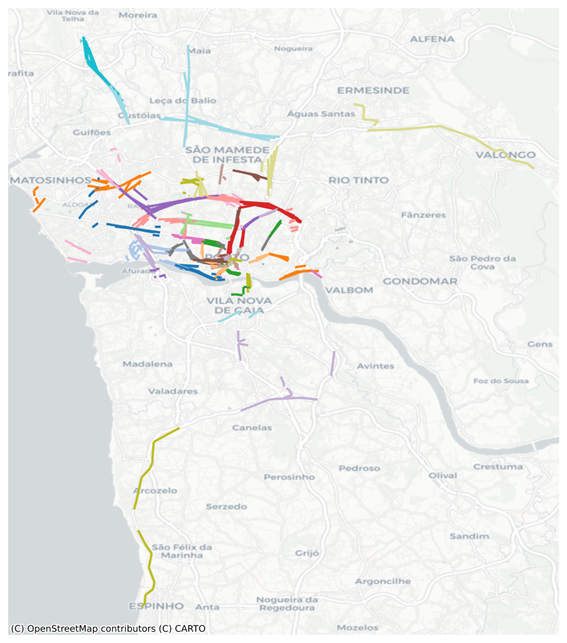
\includegraphics[width=0.5\textwidth]{img/clusters_OPTICS.png}
    \caption{Representación de clusters.}
    \label{fig:clusters_OPTICS}
\end{figure}

\begin{figure}[h!]
    \centering
    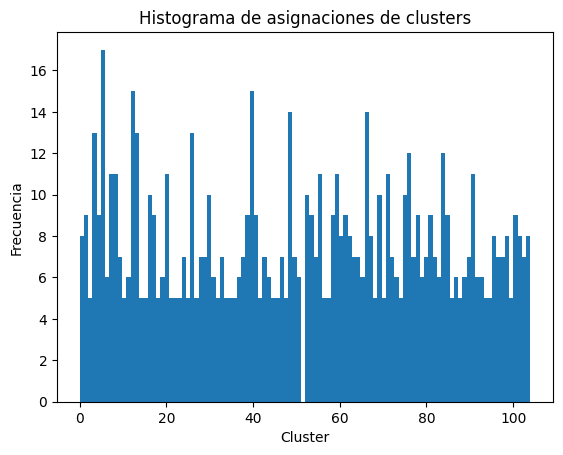
\includegraphics[width=0.5\textwidth]{img/histograma_OPTICS.png}
    \caption{Segmentos por cada cluster.}
    \label{fig:histograma_OPTICS}
\end{figure}

\begin{figure}[h!]
    \centering
    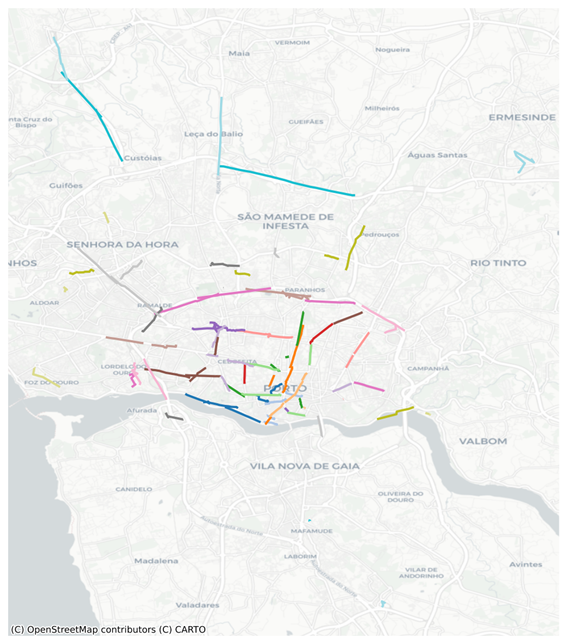
\includegraphics[width=0.5\textwidth]{img/r_tray_OPTICS.png}
    \caption{Representación de trayectorias.}
    \label{fig:trayectorias_OPTICS}
\end{figure}

\FloatBarrier

\item \textbf{DBSCAN}:  
Con un valor de \texttt{eps} de 0.1, los resultados de DBSCAN fueron significativamente diferentes a los de OPTICS. Aunque se generaron más segmentos (2654 en total), el número de clusters disminuyó a 37. Además, el porcentaje de datos clasificados como "basura" aumentó al 90.09\%, lo que equivale a 2391 segmentos descartados.

\begin{figure}[h!]
    \centering
    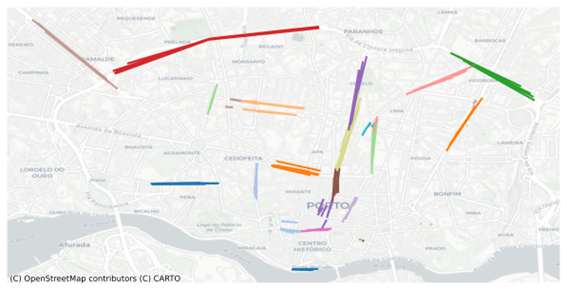
\includegraphics[width=0.5\textwidth]{img/clusters_DBSCAN.png}
    \caption{Representación de clusters.}
    \label{fig:clusters_DBSCAN}
\end{figure}

\begin{figure}[h!]
    \centering
    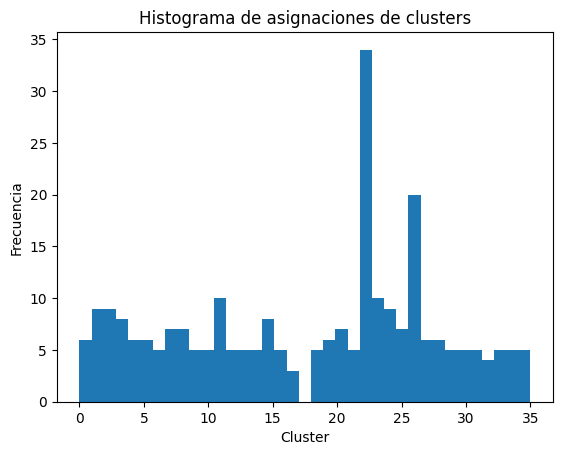
\includegraphics[width=0.5\textwidth]{img/histograma_DBSCAN.png}
    \caption{Segmentos por cada cluster.}
    \label{fig:histograma_DBSCAN}
\end{figure}

\begin{figure}[h!]
    \centering
    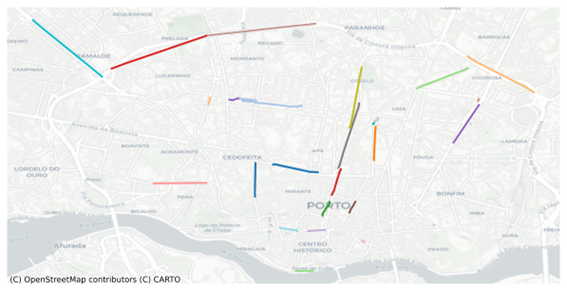
\includegraphics[width=0.5\textwidth]{img/r_tray_DBSCAN.png}
    \caption{Representación de trayectorias.}
    \label{fig:trayectorias_DBSCAN}
\end{figure}

\FloatBarrier

\item \textbf{HDBSCAN}:  
Este algoritmo no requirió ajustes en sus parámetros predeterminados de \texttt{scikit-learn}. Los resultados fueron similares a los de OPTICS en términos de segmentos (2161), aunque el número de clusters fue menor (96) y el porcentaje de segmentos descartados también disminuyó, alcanzando un 53.54\% (1157 segmentos).

\begin{figure}[h!]
    \centering
    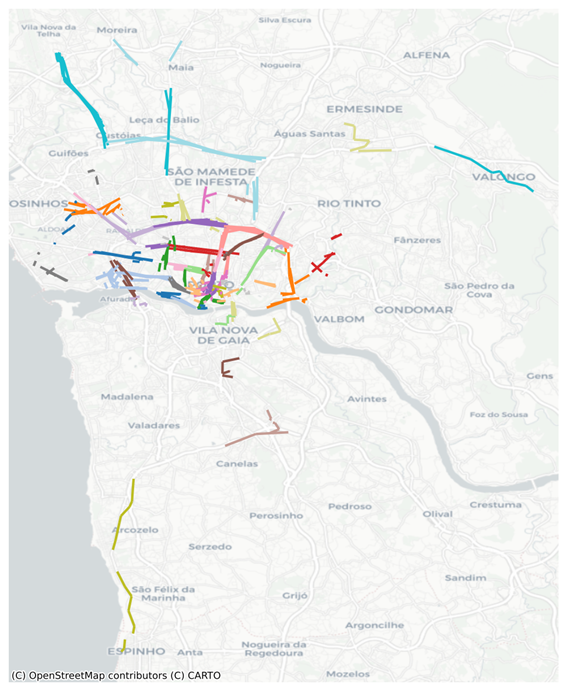
\includegraphics[width=0.5\textwidth]{img/clusters_HDBSCAN.png}
    \caption{Representación de clusters.}
    \label{fig:clusters_HDBSCAN}
\end{figure}

\begin{figure}[h!]
    \centering
    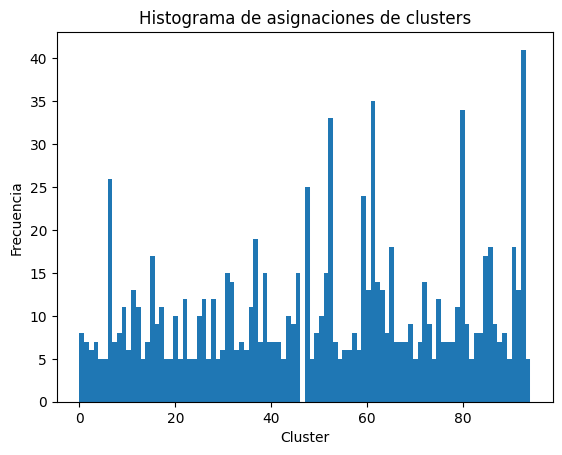
\includegraphics[width=0.5\textwidth]{img/histograma_HDBSCAN.png}
    \caption{Segmentos por cada cluster.}
    \label{fig:histograma_HDBSCAN}
\end{figure}

\begin{figure}[h!]
    \centering
    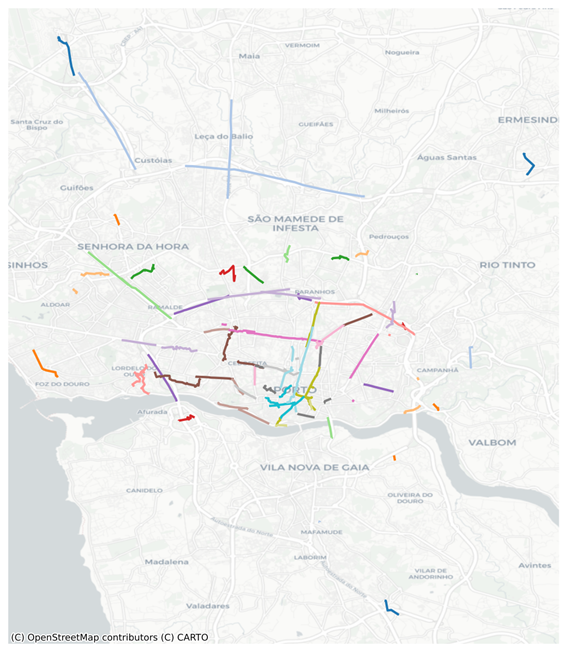
\includegraphics[width=0.5\textwidth]{img/r_tray_HDBSCAN.png}
    \caption{Representación de trayectorias.}
    \label{fig:trayectorias_HDBSCAN}
\end{figure}

\FloatBarrier

\item \textbf{Agglomerative Clustering}:  
Este algoritmo requería definir previamente el número de clusters. En este caso, se utilizaron los 2654 segmentos generados, sin descartar ninguno, ya que no clasifica datos como "basura". Sin embargo, esta característica provoca que los clusters no se centren en las zonas más densas, lo que resulta en representaciones de trayectorias más erráticas.

\begin{figure}[h!]
    \centering
    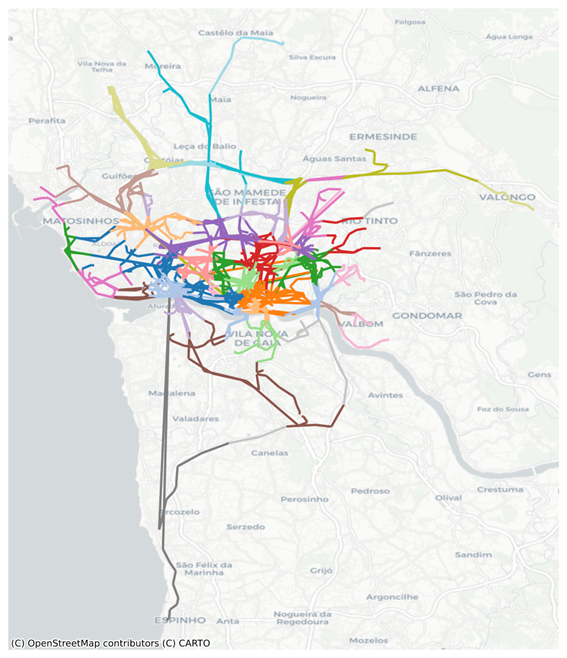
\includegraphics[width=0.5\textwidth]{img/clusters_Aggl.png}
    \caption{Representación de clusters.}
    \label{fig:clusters_Agglomerative}
\end{figure}

\begin{figure}[h!]
    \centering
    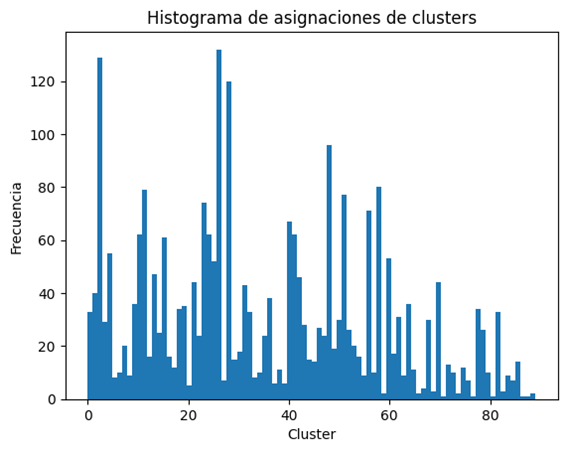
\includegraphics[width=0.5\textwidth]{img/histograma_Aggl.png}
    \caption{Segmentos por cada cluster.}
    \label{fig:histograma_Agglomerative}
\end{figure}

\begin{figure}[h!]
    \centering
    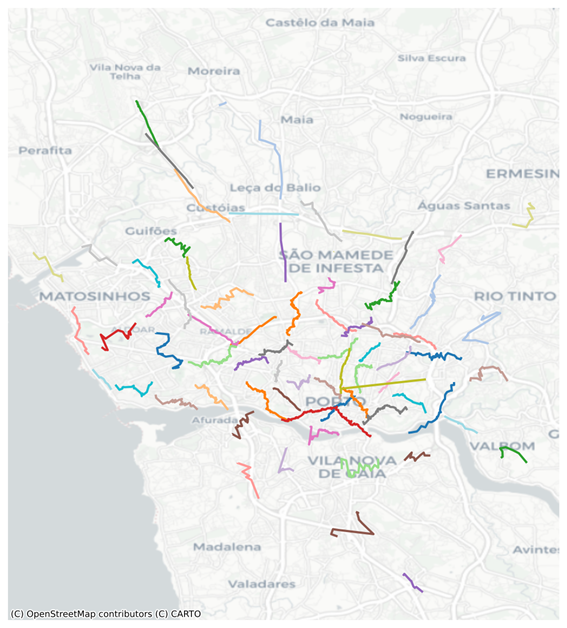
\includegraphics[width=0.5\textwidth]{img/r_tray_Aggl.png}
    \caption{Representación de trayectorias.}
    \label{fig:trayectorias_Agglomerative}
\end{figure}

\FloatBarrier

\item \textbf{Spectral Clustering}:  
Al igual que el algoritmo anterior, no descarta datos. Aunque se generaron los mismos 2654 segmentos y clusters que en Agglomerative Clustering, los resultados finales fueron diferentes, con una distribución menos centralizada.

\begin{figure}[h!]
    \centering
    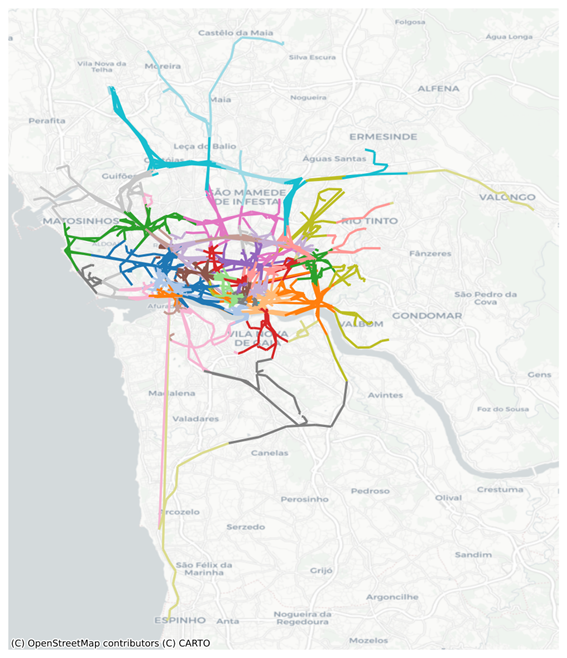
\includegraphics[width=0.5\textwidth]{img/clusters_Spect.png}
    \caption{Representación de clusters.}
    \label{fig:clusters_Spectral}
\end{figure}

\begin{figure}[h!]
    \centering
    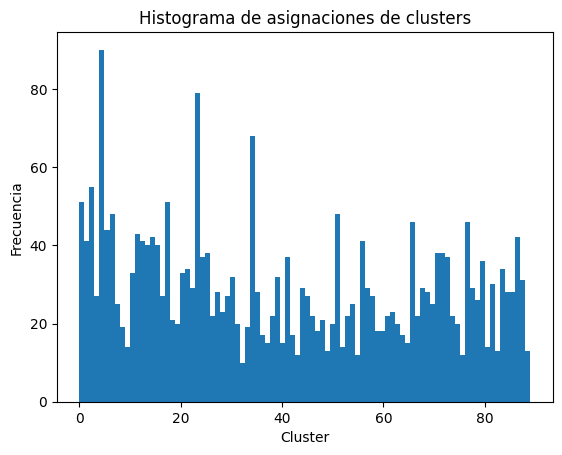
\includegraphics[width=0.5\textwidth]{img/histograma_Spect.png}
    \caption{Segmentos por cada cluster.}
    \label{fig:histograma_Spectral}
\end{figure}

\begin{figure}[h!]
    \centering
    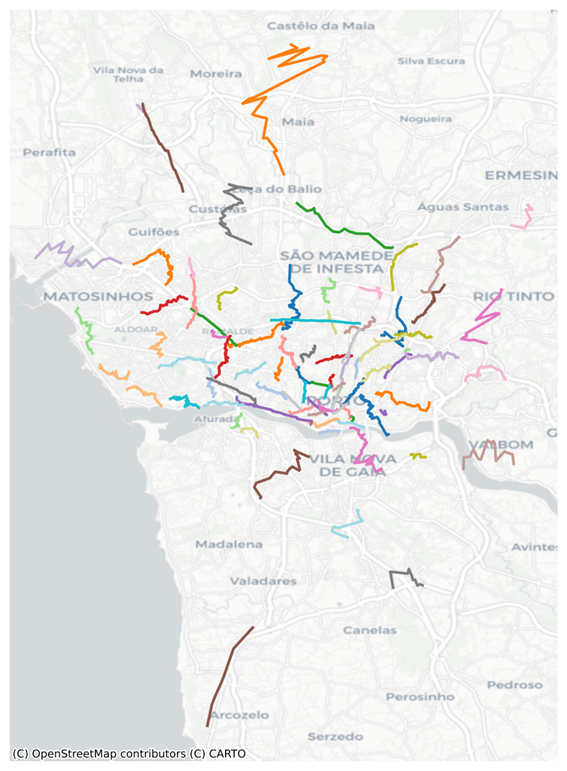
\includegraphics[width=0.5\textwidth]{img/r_tray_Spect.png}
    \caption{Representación de trayectorias.}
    \label{fig:trayectorias_Spectral}
\end{figure}

\FloatBarrier

\end{enumerate}


\section{Despliegue de la aplicación}

Para que la aplicación web funcionase correctamente y otros usuarios pudieran utilizarla, era necesario desplegarla desde el entorno local a un entorno de producción. Existen dos formas principales de realizar este proceso: crear un servidor propio o subir la aplicación a un servidor en la nube proporcionado por un tercero. Por razones económicas, se decidió optar por la segunda opción y utilizar un servidor en la nube. Para ello, se exploraron diversos servicios compatibles con aplicaciones basadas en Python.

Entre las opciones evaluadas se encontraron AWS, Azure, Heroku y Conduktor. Aunque muchas de estas plataformas ofrecían soluciones robustas con buen rendimiento, todas presentaban limitaciones económicas, ya que sus funcionalidades avanzadas suelen estar asociadas a costos recurrentes. Esto nos llevó a buscar servicios que ofrecieran una base gratuita que cubriese nuestras necesidades principales.

\subsection{Render: la solución elegida}

Tras evaluar diferentes opciones, se decidió utilizar \textbf{Render}, una plataforma que permite el despliegue de aplicaciones web, APIs y otros servicios. Render ofrece un plan gratuito que resulta ideal para proyectos pequeños o de desarrollo inicial, lo que lo convierte en una opción atractiva para aquellos con presupuestos limitados.

Render proporciona varias ventajas para aplicaciones como la nuestra:
\begin{itemize}
    \item \textbf{Compatibilidad con Python:} Es compatible con aplicaciones basadas en frameworks como Dash, Flask o Django.
    \item \textbf{Despliegue automático:} Permite integrar repositorios de GitHub o GitLab para desplegar automáticamente los cambios realizados en el código.
    \item \textbf{Certificados SSL gratuitos:} Render ofrece certificados de seguridad SSL para garantizar conexiones seguras.
    \item \textbf{Facilidad de configuración:} La plataforma cuenta con una interfaz intuitiva y bien documentada, lo que facilita el proceso de configuración incluso para usuarios con experiencia limitada en despliegues.
    \item \textbf{Soporte para aplicaciones persistentes:} Render soporta aplicaciones que requieren bases de datos o almacenamiento adicional, ideal para aplicaciones web interactivas.
\end{itemize}

\subsection{Proceso de despliegue en Render}

El despliegue de la aplicación en Render se realizó siguiendo los pasos descritos a continuación:

\begin{enumerate}
    \item \textbf{Preparación del repositorio:}
    \begin{itemize}
        \item El proyecto ya estaba alojado en un repositorio de GitHub, se incluyo un archivo \texttt{requirements.txt} que especifica las dependencias necesarias para ejecutar la aplicación.
    \end{itemize}

    \item \textbf{Creación del servicio en Render:}
    \begin{itemize}
        \item Se creó una cuenta gratuita en Render.
        \item Desde el panel de control, se seleccionó la opción \textit{"New Web Service"} y se vinculó el repositorio de GitHub al servicio.
    \end{itemize}

    \item \textbf{Configuración del entorno:}
    \begin{itemize}
        \item Se especificó el comando de inicio de la aplicación, como \texttt{python code/app/main.py}.
        \item Se configuraron las variables de entorno necesarias, como claves API o configuraciones específicas de la aplicación.
    \end{itemize}

    \item \textbf{Despliegue automático:}
    \begin{itemize}
        \item Render detectó automáticamente el contenido del repositorio y comenzó el proceso de construcción e implementación.
        \item Una vez finalizado el proceso, se asignó una URL pública para acceder a la aplicación.
    \end{itemize}

    \item \textbf{Pruebas en producción:}
    \begin{itemize}
        \item Se realizaron pruebas para verificar que todas las funcionalidades de la aplicación estuvieran operativas y que no existieran problemas relacionados con dependencias o configuración.
    \end{itemize}
\end{enumerate}

\subsection{Consideraciones finales}

Aunque Render presenta ciertas limitaciones en su plan gratuito, como tiempos de inicio más lentos para aplicaciones en estado \textit{idle} y límites de recursos, estas no afectaron significativamente a nuestra aplicación durante el desarrollo. La elección de Render permitió concentrar esfuerzos en mejorar la funcionalidad y la experiencia del usuario, sin la necesidad de invertir en infraestructura de servidor.

Con el despliegue en Render, la aplicación quedó lista para ser utilizada por cualquier usuario con acceso a Internet, cumpliendo así el objetivo de trasladar el trabajo desde un entorno local a un entorno accesible y escalable en la nube.

\section{Testing}

Para que un código sea verdaderamente funcional, seguro y mantenible, debe someterse a pruebas exhaustivas. Durante el desarrollo del proyecto, se implementaron varios tipos de pruebas para evaluar el rendimiento y la calidad del código, así como para ampliar el conocimiento en el campo del testing.

\subsection{Análisis de código estático}

El análisis de código estático es una técnica utilizada para identificar posibles errores en el código fuente sin necesidad de ejecutarlo. Este método es particularmente útil para evitar fallos humanos como bucles infinitos, errores de formato o problemas de nomenclatura.

Se evaluaron varias herramientas de análisis estático teniendo en cuenta las siguientes limitaciones:
\begin{itemize}
    \item Debían ser compatibles con Python y CSS, los lenguajes utilizados en el proyecto.
    \item No debían implicar costos adicionales.
    \item Era deseable la integración directa con GitHub para facilitar el flujo de trabajo.
\end{itemize}

Con estas características, se seleccionaron dos herramientas principales: \textbf{SonarQube} y \textbf{Code Climate}. De estas, \textbf{SonarQube} fue la más utilizada, ya que ofrecía soporte para analizar IPython Notebooks, un formato clave en los experimentos realizados durante el proyecto. Aunque los notebooks no formaban parte directa de la aplicación web, su análisis fue crucial para garantizar la calidad de los experimentos previos.

Lo ideal en este tipo de análisis es aplicarlo de manera continua durante las diversas fases del proyecto, ya que esto reduce significativamente la carga de trabajo y mejora la calidad del código a medida que se desarrolla. Sin embargo, en este proyecto, el análisis estático se realizó al final, lo que no fue óptimo pero permitió identificar una serie de problemas, entre ellos:

\begin{itemize}
    \item \textbf{Mejoras en nomenclatura:} Se ajustaron nombres de variables para facilitar su comprensión y evitar confusiones con otros datos.
    
\begin{figure}[h!]
    \centering
    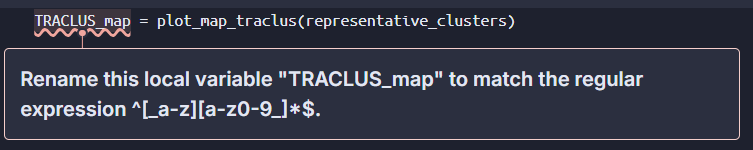
\includegraphics[width=0.5\textwidth]{img/sonarq_regularexp.png}
    \caption{Error nomenclatura.}
    \label{fig:trayectorias_Spectral}
\end{figure}    
    
    \item \textbf{Variables no utilizadas:} Se detectaron y eliminaron variables que ya no eran relevantes, ya fuera por errores en su definición o por haber quedado obsoletas durante el desarrollo.
    
\begin{figure}[h!]
    \centering
    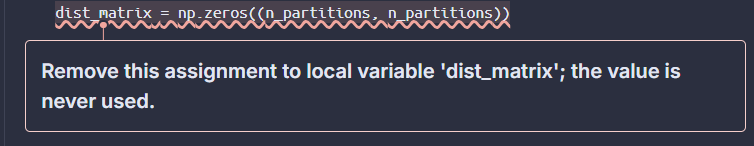
\includegraphics[width=0.5\textwidth]{img/sonarq_codigo_sobrante.png}
    \caption{Código innecesario.}
    \label{fig:trayectorias_Spectral}
\end{figure}

\begin{figure}[h!]
    \centering
    
\includegraphics[width=0.5\textwidth]{img/sonarq_unused.png}
    \caption{Variable sin usar necesaria.}
    \label{fig:trayectorias_Spectral}
\end{figure}    
    
    \item \textbf{Importaciones innecesarias:} Se eliminaron módulos y librerías no utilizadas, lo que ayudó a reducir la carga del programa y mejorar su legibilidad.
    
\begin{figure}[h!]
    \centering
    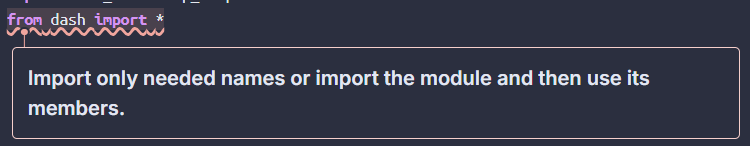
\includegraphics[width=0.5\textwidth]{img/sonarq_imports.png}
    \caption{Importación excesiva.}
    \label{fig:trayectorias_Spectral}
\end{figure}
   
    \item \textbf{Complejidad en funciones:} Se identificaron funciones cuya complejidad excedía los límites recomendados. Aunque algunas de estas funciones no pudieron simplificarse debido a las características del algoritmo, el análisis ayudó a priorizar futuras mejoras.
    
\begin{figure}[h!]
    \centering
    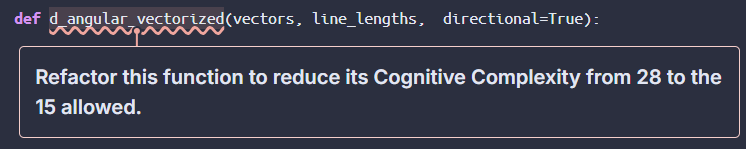
\includegraphics[width=0.5\textwidth]{img/sonarq_complex.png}
    \caption{Complejidad grande.}
    \label{fig:trayectorias_Spectral}
\end{figure}

\end{itemize}

Aunque este tipo de análisis no corrige directamente errores en la funcionalidad del algoritmo, resulta muy útil para evitar problemas menores, mejorar la mantenibilidad del código y garantizar un nivel básico de seguridad.

\subsection{Pruebas unitarias}

Las pruebas unitarias son fundamentales para garantizar la funcionalidad de cada componente del código. Estas pruebas...




\capitulo{6}{Trabajos relacionados}

Este apartado sería parecido a un estado del arte de una tesis o tesina. En un trabajo final grado no parece obligada su presencia, aunque se puede dejar a juicio del tutor el incluir un pequeño resumen comentado de los trabajos y proyectos ya realizados en el campo del proyecto en curso. 

\capitulo{7}{Conclusiones y Líneas de trabajo futuras}

Todo proyecto debe incluir las conclusiones que se derivan de su desarrollo. Éstas pueden ser de diferente índole, dependiendo de la tipología del proyecto, pero normalmente van a estar presentes un conjunto de conclusiones relacionadas con los resultados del proyecto y un conjunto de conclusiones técnicas. 
Además, resulta muy útil realizar un informe crítico indicando cómo se puede mejorar el proyecto, o cómo se puede continuar trabajando en la línea del proyecto realizado. 



\bibliographystyle{plain}
\bibliography{bibliografia}

\end{document}
